%This chapter considers one of the supporting algorithms for sketch-based modeling system introduced in Chapter~\ref{ch:planeSBIM} -- the surface-based mesh deformation algorithm. Surface deformation for triangular meshes has become a popular research topic in computer graphics and geometric modeling. Most of the existing mesh deformation methods establish their formulations in the primal vertex-based domain and are expected to produce globally smooth and consistent deformation results while preserving geometry details as much as possible. In this chapter, we present a new surface-based mesh deformation method that performs the computation via an edge-based graph to increase the sampling rate for more accurate shape computation and better deformation results. The user is given the flexibility of adjusting the deformation effect between local shape preservation and global smoothness. Moreover, to simulate the deformation behaviors of regions with different materials, we introduce a stiffness property into the deformation model and present an easy and intuitive way for the user to set the material property. Experimental results demonstrate that our algorithm can produce satisfactory results and make the deformation more flexible.
This chapter presents an edge-based flexible mesh deformation
algorithm, which effectively supports the deformation function in
our sketch-based modeling system.

%=================section==================
\section{Introduction}
\label{ch5:sec:intro}
%==========================================
Mesh deformation is an effective and convenient  method for mesh
editing in geometric modeling and computer animation, and it is also
an important sculpting function in sketch-based modeling systems. It
allows the user to manipulate one part or the entire surface while
preserving some geometric characteristics of the initial surface. As
 introduced in Section~\ref{ch2:sec:deformation}, various
algorithms on mesh deformation have been developed due to its
importance and popularity in a wide rage of applications in
industrial and artistic designs. Though having their respective
advantages, those algorithms also have drawbacks due to the
following considerations in mesh deformation.

First, a triangular mesh is a piecewise linear  surface and it is
often considered as an approximation of some unknown smooth surface.
The approximation effect is related to the number of vertices of the
mesh. In general, the larger the number of vertices the mesh
contains, the better is the approximation. When a deformation is
performed on a surface, the calculation will be conducted on the
vertices. The number of vertices determines the sampling rate in
approximating a continuous model and thus a denser mesh usually
results in more accurate deformation. However, given a deformation
region, the number of vertices is fixed and it is not trivial to
have more points be involved in the deformation calculation.

Second, in the deformation process the local  shape feature is often
required to be well preserved and the deformed shape should be
natural and smooth to satisfy aesthetics or other requirements. A
natural problem then arises: what is a good balance between the
rigidity and fairness? The answer is subjective. A satisfactory
editing result depends on the algorithm adopted, the specific models
and the desired effect as well.

Third, an object in real world may be  composed of different
materials, which may exhibit different behaviors when the object is
deformed. For example, with different stiffness properties of the
materials, different deformation effects between rigidity and
smoothness will appear under the deformation. Most of the existing
deformation methods are purely geometrically-based and they ignore
the material properties of the object.

To solve these problems and make the  deformation more flexible, we
propose a flexible mesh deformation algorithm which performs the
computation through an edge-based graph. Instead of formulating the
deformation on the primal domain, we build an edge-based graph and
carry out the deformation computations on the graph, which involves
more nodes and thus produces better deformation results. We then
propose a mixed energy model that combines the first order and the
second order discrete differential quantities to balance local shape
preservation and smoothness. The user can adjust the values of the
balance parameter to control the deformation results. Moreover,
these introduced balance parameters are used to reflect the
stiffness property of the object material and thus make the
deformation algorithm material-aware. A simple sketching tool is
provided to specify the stiffness property. The novelty of the
chapter thus lies in the use of the edge-based graph for the
deformation formulation and the use of balance parameters for
controlling the stiffness and producing various reasonable
deformation results in a mesh deformation task.



%==========================================
\section{Edge-based graph} \label{ch5:sec:alg:edgegraph}
Let
$M=(V,E)$ be a triangular mesh with $n$ vertices. $V=\{v_i|v_i\in
R^3,i=1,...,n\}$ denotes the set of vertices and
$E=\{e_{ij}=(v_i,v_j)|v_i,v_j\in V,i\neq j\}$ represents the set of
edges. Correspondingly, we define $\tilde{M}=(\tilde{V},\tilde{E})$
as the corresponding edge-based graph for $M$, where
$\tilde{V}=\{\tilde{v_i}|\tilde{v_i}\in R^3,i=1,...,n_e\}$ and
$\tilde{E}=\{\tilde{e_{ij}}=(\tilde{v_i},\tilde{v_j})|\tilde{v_i},\tilde{v_j}\in
\tilde{V},i\neq j\}$ are the sets of nodes and edges of the
edge-based graph respectively. Specifically, a node $\tilde{v_i}$ is
defined as the midpoint of the edge $e_{ij}$  in the primal domain:
$\tilde{v_i}=(v_i+v_j)/2$. $n_e$ represents the number of nodes in
the edge-based graph, which equals the number of edges on the primal
mesh $M$. Each node $\tilde{v_i}$ corresponding to primal edge
$e_{ij}$ is connected to four neighboring nodes corresponding to the
four primal edges that share the vertices of $e_{ij}$. In this way,
the valence of each node in the edge-based graph is always four. The
conversion from the primal vertex positions $V$ to the edge-based
graph vertex positions $\tilde{V}$ can be accomplished by an
$n_e\times n$ sparse matrix $D$. Each row of $D$ has two non-zero
elements that are 1/2. Figure~\ref{fig:edgebasedgraph} shows an
edge-based graph constructed from a primal mesh.

\begin{figure} [htbp]
    \centering
  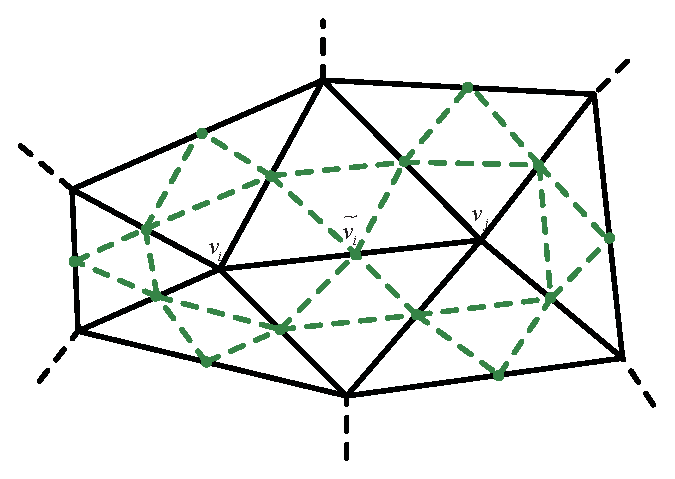
\includegraphics[scale=0.6]{figs/f5.2.edge-based-graph.eps}
  \caption{An illustration of an edge-based graph. The black lines represent the primal mesh and the green lines form the edge-based graph.}
  \label{fig:edgebasedgraph} %% label for entire figure
\end{figure}



%==========================================
\section{Flexible mesh deformation} \label{ch5:sec:alg:flexdefo}
In  mesh deformation, the user first  specifies the \textit{handle}
vertices and their new positions, as well as the \textit{static}
vertices that will remain unchanged, and then the algorithm
determines the deformation of the \textit{region-of-interest (ROI)}
vertices. Many previous deformation algorithms aim to preserve
either the first or the second order discrete differential
quantities of the mesh surface and thus can produce only one kind of
deformation result, which may be either too rigid or smooth.

We present  a method that considers both of the two differential
quantities and balances between the rigidity and smoothness of the
deformation in a flexible manner. Our basic idea is to deform the
vertices in the ROI such that a mixed energy functional is minimized
and this minimization problem is formulated on an edge-based graph.
The mixed energy functional includes the change of the first order
and second order differential quantities that reflect stretching and
bending. Based on Euler-Poincare formula, the number of edges on a
triangular mesh is approximately three times that of vertices. Thus
the energy functional formulated on the edge-based graph better
approximates the continuous version of the energy functional of the
smooth surface than that on the primal domain. Thus the formulation
on the edge-based graph tends to render better deformation results,
especially when rigid or smooth deformation effects are required.
See Figure~\ref{fig:deformbaby} for an example.

\begin{figure} [htbp]
  \centering
  \subfigure[]{
    \centering
    \label{fig:deformbaby:a} %% label for first subfigure
    \begin{minipage}[b]{0.3\textwidth}
      \centering
      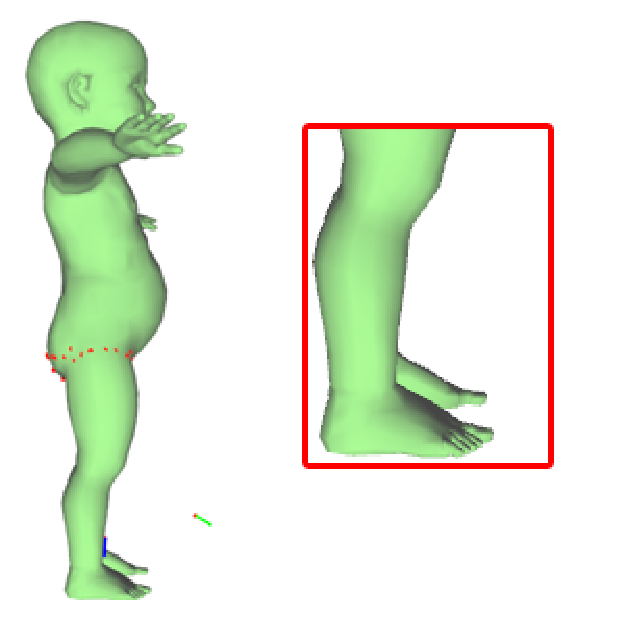
\includegraphics[scale=0.35]{figs/f5.1.baby-pc-3.eps}
    \end{minipage}}
   \\
  \subfigure[]{
    \centering
    \label{fig:deformbaby:b}
    \begin{minipage}[b]{0.3\textwidth}
      \centering
      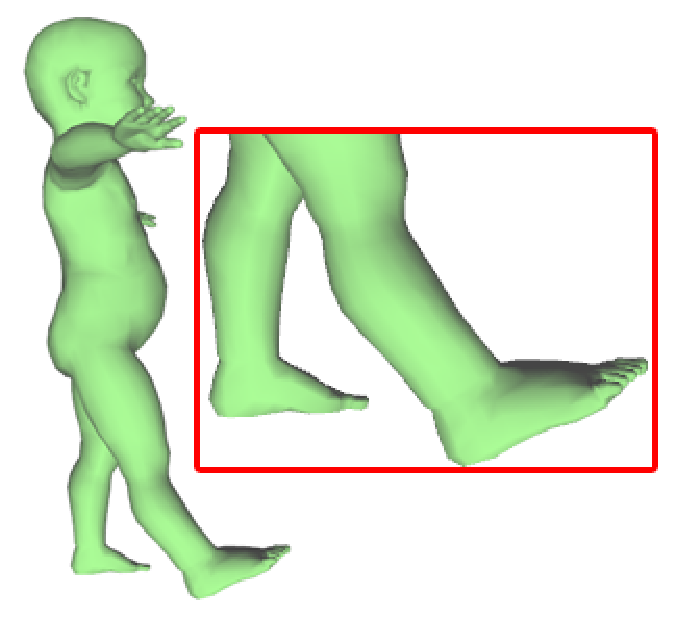
\includegraphics[scale=0.35]{figs/f5.1.ver0-iso-3.eps}
    \end{minipage}}
  \subfigure[]{
    \centering
    \label{fig:deformbaby:c}
    \begin{minipage}[b]{0.3\textwidth}
      \centering
      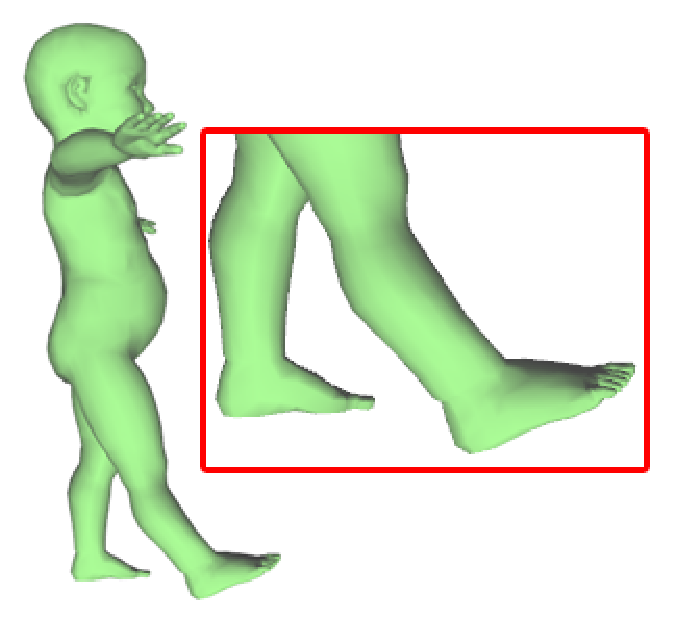
\includegraphics[scale=0.35]{figs/f5.1.ver05-iso-3.eps}
    \end{minipage}}
  \subfigure[]{
    \centering
    \label{fig:deformbaby:d}
    \begin{minipage}[b]{0.3\textwidth}
      \centering
      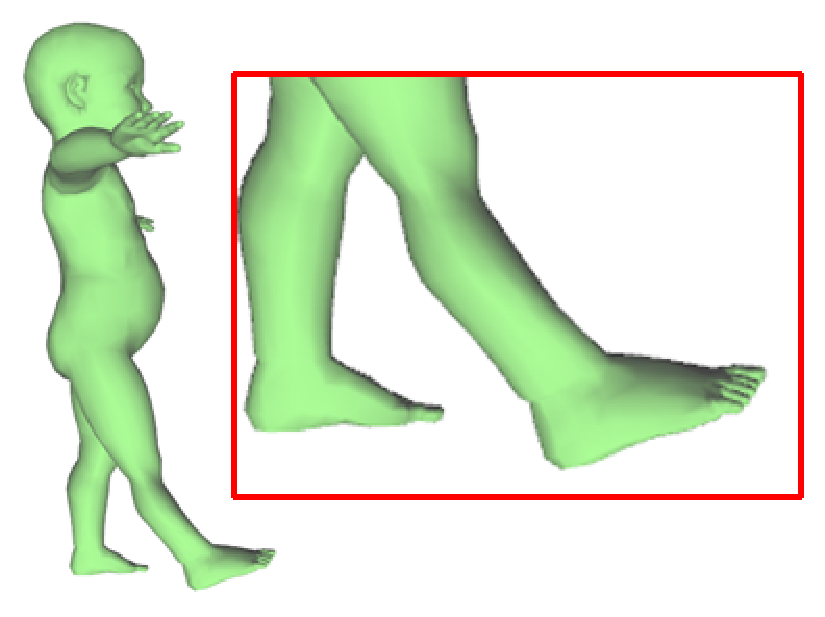
\includegraphics[scale=0.35]{figs/f5.1.ver10-iso-3.eps}
    \end{minipage}}
  \\
  \subfigure[]{
    \centering
    \label{fig:deformbaby:e} %% label for first subfigure
    \begin{minipage}[b]{0.3\textwidth}
      \centering
      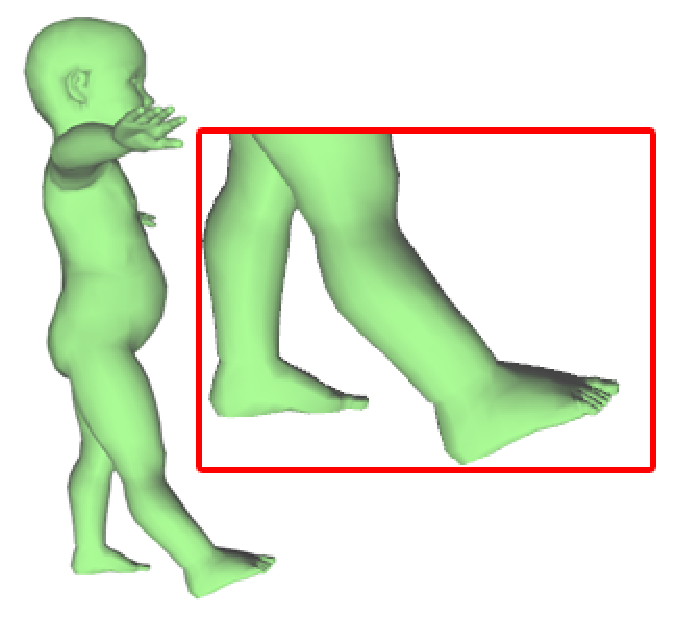
\includegraphics[scale=0.35]{figs/f5.1.edge0-iso-3.eps}
    \end{minipage}}
  \subfigure[]{
    \centering
    \label{fig:deformbaby:f}
    \begin{minipage}[b]{0.3\textwidth}
      \centering
      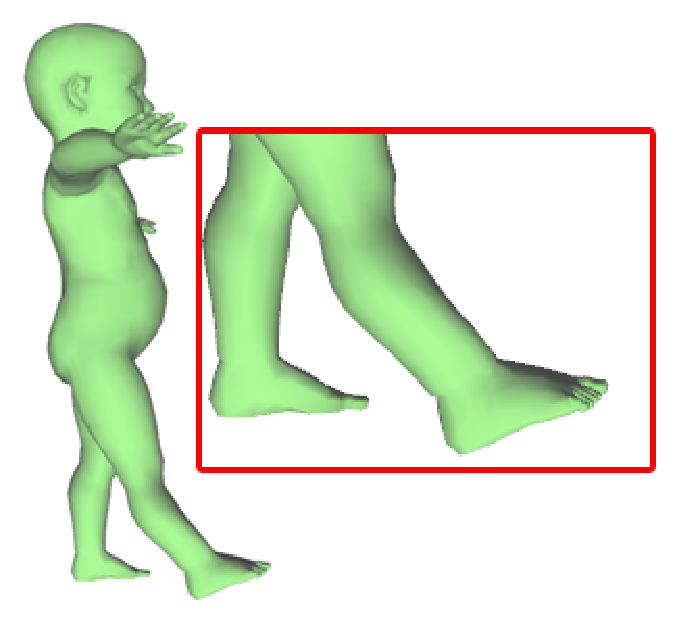
\includegraphics[scale=0.35]{figs/f5.1.edge05-iso-3.eps}
    \end{minipage}}
  \subfigure[]{
    \centering
    \label{fig:deformbaby:g}
    \begin{minipage}[b]{0.3\textwidth}
      \centering
      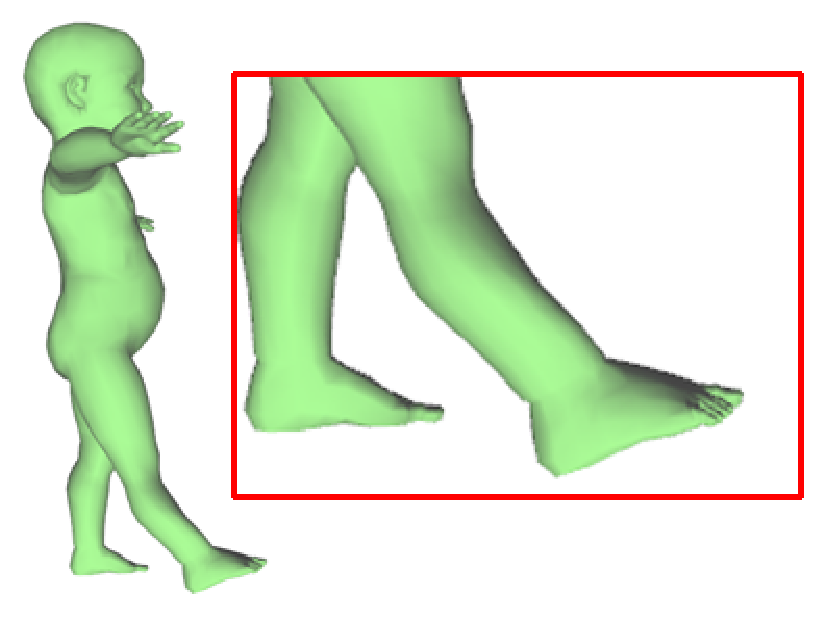
\includegraphics[scale=0.35]{figs/f5.1.edge10-iso-3.eps}
    \end{minipage}}
  \caption{Flexible deformation of the \textit{Baby} model. (a) The initial model. (b)-(d) Results of the flexible deformation algorithm performed on the primal domain, with the global balance parameters valued 0, 0.5 and 1.0 respectively. (e)-(g) Results of the flexible deformation algorithm performed via the edge-based graph, with the global balance parameters valued 0, 0.5 and 1.0 respectively.}
  \label{fig:deformbaby} %% label for entire figure
\end{figure}






%==========================================
\subsection{First and second order discrete differential
quantities} First of all we need to find proper  representations for
the first and second order discrete differential quantities of the
mesh surface.

For a smooth surface, the  first order differential properties are
usually represented by length, area, etc. However, these will make
the system nonlinear. So for triangular meshes we choose to use edge
vectors at each node, which we called the 1-form, to represent the
first order differential structures of the mesh surface. The 1-form
contains the information of edge lengths and can help to make the
final system a linear one.

Specifically, for a  node $\tilde{v_i}$, the 1-form can be
represented by the edge vectors $\tilde{e_{ij}}$ which start from
the one-ring neighborhood $\tilde{v_j},\tilde{e_{ij}}\in \tilde{E}$
and point to $\tilde{v_i}$, as shown in
Figure~\ref{fig:edgebasedoneform}. It can totally decide the shape
of the local area around a node. That is to say, as long as the edge
vectors connecting $\tilde{v_i}$ and its neighbors are fixed, the
shape of the local area around $\tilde{v_i}$ is fixed.

The second order differential properties of  a smooth surface are
usually represented by curvatures, which also make the system a
nonlinear one~\cite{ESP08}. The Laplacian vector provides a proper
choice for representing the second order differential properties of
the mesh surface, since its magnitude approximates the mean
curvature at each vertex and the final system formed is a linear
one. So we extend the traditional definition of Laplacian vector
from the primal mesh to the edge-based graph and use it to represent
the second order discrete differential quantity of the mesh surface,
as shown in Figure~\ref{fig:edgebasedlap}.

\begin{figure} [htbp]
  \subfigure[]{
    \centering
    \label{fig:edgebasedoneform}
    \begin{minipage}[b]{0.45\textwidth}
      \centering
      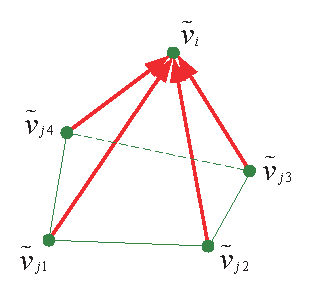
\includegraphics[scale=0.8]{figs/f5.3.Rigid.eps}
    \end{minipage}}
  \subfigure[]{
    \centering
    \label{fig:edgebasedlap}
    \begin{minipage}[b]{0.45\textwidth}
      \centering
      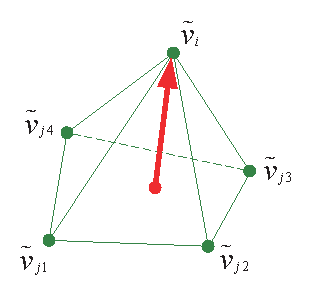
\includegraphics[scale=0.8]{figs/f5.3.Laplacian.eps}
    \end{minipage}}
  \caption{(a) The 1-form. (b) The Laplacian vector.}
  \label{fig:edgebasedoneformlap} %% label for entire figure
\end{figure}

Mathematically, the Laplacian vector $\tilde{\delta_i}$ at $\tilde{v_i}$ is defined as:

\begin{equation}
\label{eq:edgelaplacian}
\tilde{\delta_i}=L(\tilde{v_i})=\sum\limits_{j\in N(i)}{\tilde{\omega_{ij}} (\tilde{v_i}-\tilde{v_j})},
\end{equation}
where $N(i)=\{j|\tilde{e_{ij}}\in \tilde{E}\}$ is the  index set of
adjacent nodes in the neighboring ring of $\tilde{v_i}$ and
$\tilde{\omega_{ij}}$ is the weight of the edge $\tilde{e_{ij}}$.
Here we use the cotangent weight scheme~\cite{MDSB02} to compute
$\tilde{\omega_{ij}}$. In fact, $L(\cdot)$ can be regarded as the
discretized Laplace-Beltrami operator with cotangent coefficients on
triangular meshes~\cite{BS08}.

It should be noted that the Laplacian  vector $\tilde{\delta_i}$ in
the edge-based graph can also be regarded as a measurement of the
dihedral angle $\alpha_i$ of two adjacent triangles in the primal
mesh, which also represents the second order differential property
of the mesh surface. The magnitude of $\tilde{\delta_i}$ is
inversely proportional to the size of $\alpha_i$, as can be seen in
Figure~\ref{fig:edgebaseddihedral}.

\begin{figure} [htbp]
  \subfigure[]{
    \centering
    \label{fig:edgebaseddihedral1}
    \begin{minipage}[b]{0.45\textwidth}
      \centering
      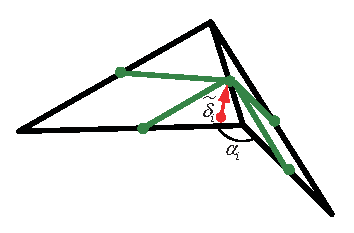
\includegraphics[scale=0.8]{figs/f5.4.dihedral1.eps}
    \end{minipage}}
  \subfigure[]{
    \centering
    \label{fig:edgebaseddihedral2}
    \begin{minipage}[b]{0.45\textwidth}
      \centering
      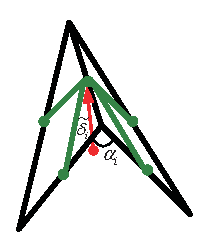
\includegraphics[scale=0.8]{figs/f5.4.dihedral2.eps}
    \end{minipage}}
  \caption{The Laplacian vector $\tilde{\delta_i}$ in the edge-based graph and the dihedral angle $\alpha_i$ between adjacent faces in the primal domain. (a) The shorter $\tilde{\delta_i}$ is, the larger $\alpha_i$ will be. (b) The longer $\tilde{\delta_i}$ is, the smaller $\alpha_i$ will be. }
  \label{fig:edgebaseddihedral} %% label for entire figure
\end{figure}

These two representations  of discrete differential quantities
encode the relative position of each node w.r.t. its neighboring
nodes and represent the local geometry properties of the mesh
surface. Next we will introduce how to combine them to get a
satisfactory deformation result flexibly.

%==========================================
\subsection{Energy function for flexible deformation} The approach
for solving  the deformation problem of the surface-based method is
to designate the positional constraints for the handle and static
vertices and solve for the positions of the ROI vertices by fitting
the local geometry properties of the deformed mesh to those of the
initial mesh. The properties we want to preserve include both the
first and second order discrete differential properties, which are
represented by the 1-form and Laplacian vectors.

Since the 1-form at each node $\tilde{v_i}$ can  totally decide the
shape of a local neighborhood area, it is considered as defining the
local shape of the mesh surface in a unique manner. Mathematically,
to preserve the 1-form of the initial mesh, the energy we try to
minimize for each node $\tilde{v_i}$ is:

\begin{equation}
\label{eq:edgerigidenergy}
E(\tilde{v_i}^\prime)=\sum\limits_{j\in N(i)}{\tilde{\omega_{ij}} ||\tilde{e_{ij}}^\prime -R_i \tilde{e_{ij}}||^2},
\end{equation}
where $\tilde{v_i}^\prime$ is the new  position of $\tilde{v_i}$,
$\tilde{e_{ij}}=\tilde{v_i}-\tilde{v_j}$ and
$\tilde{e_{ij}}^\prime=\tilde{v_i}^\prime-\tilde{v_j}^\prime$ are
the undeformed and deformed edge vectors between $\tilde{v_i}$ and
$\tilde{v_i}$ respectively. $\tilde{\omega_{ij}}$ is the same weight
as that in Eq.~\ref{eq:edgelaplacian}. $R_i$ represents the rotation
matrix associated to $\tilde{v_i}$. The optimal rotation matrix
$R_i$ can be calculated given the old and new values of the edge
vectors. Detailed deduction can be found in~\cite{SA07}.

The rigid transformation of the 1-form during  deformation strives
to do a \textit{hard} transform to the mesh. We say \textit{hard} as
the edge vectors of each node can completely determine the shape of
its neighborhood area. As long as each vector keeps fixed, the shape
of this area will not change at all.

To preserve each Laplacian vector of the mesh  surface during
deformation, we try to minimize its change up to an affine
transformation $T_i$. Since shearing and anisotropic scale will lead
to distortions of the local features~\cite{FAT07}, we assume $T_i$
be composed of rotation and isotropic scale, i.e. $T_i=s_iR_i$.
$s_i$ and $R_i$ represent the scale coefficient and rotation matrix
separately. The energy to minimize is:

\begin{equation}
\label{eq:edgelapenergy}
E(\tilde{v_i}^\prime)=||\sum\limits_{j\in N(i)}{\tilde{\omega_{ij}}(\tilde{v_i}^\prime - \tilde{v_j}^\prime)} -T_i\sum\limits_{j\in N(i)}{\tilde{\omega_{ij}}(\tilde{v_i} - \tilde{v_j})}||^2.
\end{equation}

The deformation of preserving the Laplacian vectors  is a relatively
\textit{soft} deformation, comparing to the hard one, since the
Laplacian vector cannot exactly represent the shape of the local
area around each node. The word \textit{soft} has another meaning
that the deformed shape tends to be smooth, since the change of the
second order differential quantity is minimized to prevent the sharp
change of the mesh shape within a local area.

Up to now, we have obtained two linear methods for  mesh deformation
by preserving the 1-form and Laplacian vectors respectively. The
unknowns in the two systems are both the set of deformed node
positions. However, neither of the two methods can satisfy our
requirement of obtaining various deformation effects between
rigidity and smoothness. In the first method, while the
representation of the local shape is quite accurate, sometimes the
deformation will be too rigid that smoothness cannot be obtained.
Besides, a definite rigid transformation means that scale is not
considered, and thus some local features cannot be preserved under
this kind of transformation. In the second method, since the
Laplacian vector cannot exactly represent the shape of a local
region, local shape preservation may not be achieved. However, the
deformation calculated using this method is relatively smooth.
Moreover, scale transformation is considered in the computation to
make the result more natural and help to preserve the local features
under stretching or shrinking.

To make use of the advantages of these two methods and  give the
user flexibilities to choose the most desirable deformation effect
between rigidity and smoothness subject to a specific model, we
propose a new algorithm which combines the two methods using a
balance parameter $\lambda$. When $\lambda=1$, only the first order
discrete differential quantity of each node is preserved and the
deformation is the most rigid; when $\lambda=0$, only the second
order discrete differential quantities are preserved and a smooth
result is achieved. Multiple intermediate results can be obtained by
setting different $\lambda$ values between 0 and 1.

Considering the positional  constraints $\{\tilde{c_i}\},i\in
\{m,...,n\},m<n$, the overall energy we aim to minimize for a mesh
deformation task with $n$ nodes involved is:

\begin{eqnarray}
\label{eq:edgelocflexenergy}
E(V^\prime) &=& \sum\limits_{i=1}^n{\lambda_i(\sum\limits_{j\in N(i)}{\tilde{\omega_{ij}} ||\tilde{e_{ij}}^\prime -R_i \tilde{e_{ij}}||^2})}+\nonumber\\
& & \sum\limits_{i=1}^n{(1-\lambda_i)||\sum\limits_{j\in N(i)}{\tilde{\omega_{ij}}(\tilde{v_i}^\prime - \tilde{v_j}^\prime)} -T_i\sum\limits_{j\in N(i)}{\tilde{\omega_{ij}}(\tilde{v_i} - \tilde{v_j})}||^2}+\nonumber\\
& &\sum\limits_{i=m}^n{||\tilde{v_i}^\prime-\tilde{c_i}||^2},
\end{eqnarray}
in which the first and second  items of the right hand side are the
energies measured by the change of the 1-form and Laplacian vectors
and the third item is the positional constraints during deformation.
The balance parameter $\lambda_i (0\leq \lambda_i\leq 1)$ is used to
control the rigidity and smoothness of the deformation at node
$\tilde{v_i}$.

It is not difficult to see that the definitions  of 1-form and
Laplacian vectors and the flexible deformation algorithm can be
easily transferred to the primal domain, by replacing the variables
defined in the edge-based graph in Eq.~\ref{eq:edgelocflexenergy}
with those of the primal domain. This is useful for comparing the
deformation results calculated directly in the primal domain and via
the edge-based graph. Detailed comparisons can be found in
Section~\ref{ch5:sec:results}.


%==========================================
\subsection{Solving of the system} To solve this system, we use an
iterative method  which can be outlined as follows.

First we build an edge-based graph for the  deformation region of
the mesh and then compute the partial derivatives of the first and
second items in energy function~\ref{eq:edgelocflexenergy} w.r.t.
the unknown node positions $\tilde{V}^\prime$ and get two linear
systems $A_1\tilde{V}^\prime=b_1$ and $A_2\tilde{V}^\prime=b_2$. An
important observation is that if the coefficients $\lambda_i$ and
$1-\lambda_i$ are not considered, $A_1$ and $A_2$ happen to be the
same. So only one of them needs to be constructed in the beginning
and we just need to focus on the calculation of the right hand side
of the system in each iteration.

Then an initial deformation result is  estimated using the naive
Laplacian deformation~\cite{AM01} which does not consider rotation
and scale transformations of the Laplacian vectors. Based on the
estimated vertex positions, we can compute the rotation matrix $R_i$
and the transformation matrix $T_i$. Since the optimal $R_i$ can be
uniquely calculated through singular value
decomposition~\cite{SA07}, we make use of it to compute the optimal
scale coefficient $s_i$, such that $T_i=s_iR_i$ can be obtained.
This way, computations of $R_i$ and $T_i$ are associated and the
overall calculation process is accelerated. The right hand side of
the system is then updated by multiplying the calculated $R_i$ and
$T_i$ and the system can be solved.

Next some iterations are performed for  recomputing $R_i$ and $T_i$,
updating the right hand side of the system and solving it. This
process continues until convergence.

As all the above computations are  performed in the edge-based
graph, we need to reconstruct the primal mesh by using the
conversion matrix $D$ introduced in
Section~\ref{ch5:sec:alg:edgegraph} as well as the positional
constraints for primal handle and static vertices. However, since
the position of each node in the edge-based graph can be represented
as the linear combination of two primal vertex positions, an easier
way to solve the system is to integrate $D$ into
Eq.~\ref{eq:edgelocflexenergy} and directly take the primal vertex
positions as unknowns.



%==========================================
\section{Specification of the balance parameters}

In the preceding section we assume that the  balance parameters have
been predefined and treat them as constants during the calculation.
Now we  provide two methods to specify the balance parameters: a
global method and a local method.

In the global method, we let the  balance parameter $\lambda_i$ for
each node $\tilde{v_i}$ equal to the same value $\lambda$, such that
energy function~\ref{eq:edgelocflexenergy} turns to:

\begin{eqnarray}
\label{eq:edgeglbflexenergy}
E(V^\prime) &=& \lambda\sum\limits_{i=1}^n{(\sum\limits_{j\in N(i)}{\tilde{\omega_{ij}} ||\tilde{e_{ij}}^\prime -R_i \tilde{e_{ij}}||^2})}+\nonumber\\
& & (1-\lambda)\sum\limits_{i=1}^n{||\sum\limits_{j\in N(i)}{\tilde{\omega_{ij}}(\tilde{v_i}^\prime - \tilde{v_j}^\prime)} -T_i\sum\limits_{j\in N(i)}{\tilde{\omega_{ij}}(\tilde{v_i} - \tilde{v_j})}||^2}+\nonumber\\
& &\sum\limits_{i=m}^n{||\tilde{v_i}^\prime-\tilde{c_i}||^2}.
\end{eqnarray}

This global method provides a  proper choice when the user wants to
make the entire editing region of a mesh deform in a consistent
manner. The rigidity and smoothness of the deformation can be well
balanced through setting a proper $\lambda$ value between 0 and 1.
The user can select a proper $\lambda$ value to produce a
satisfactory result, according to the specific model and the
deformation effect he needs. Generally speaking, larger $\lambda$
values make the deformation more rigid and smaller $\lambda$ values
make it more fair. It can be seen that previous methods which
preserve either the first or the second order differential
properties of the mesh surface is just a special case of
Eq.~\ref{eq:edgeglbflexenergy}.

Examples of the global method  can be seen in
Figures~\ref{fig:deformdino} to~\ref{fig:deformJCglb}.

Although the global method  provides an efficient way of calculating
a natural and consistent deformation result for the entire editing
region, it ignores the individual property of each local area on the
mesh surface and sometimes is not flexible. So we also provide a
local method for the specification of the balance parameters.

Since objects in the real world  are often composed of non-uniformly
distributed materials, their deformation behaviors vary from
rigidity to smoothness across the surface, depending on the
stiffness of the materials on each local region. However, current
mesh deformation algorithms either ignore the underlying materials
of the mesh surface or suffer various problems. The physics or
skeleton based algorithms provide feasible approaches to solve this
problem. Nevertheless, they are either slow in computation or
limited to a subset of models~\cite{PJS05}.

Since the balance parameter can be used to  control the rigidity and
smoothness of the deformation, we can use it to define the stiffness
property of the material on each local area of the mesh surface,
such that the regions with different materials will have
distinguished behaviors in a same deformation task. In this case,
$\lambda_i$ for each $\tilde{v_i}$ in Eq.~\ref{eq:edgelocflexenergy}
should be defined separately according to the material property of
$\tilde{v_i}$. The larger $\lambda_i$ is, the stiffer the material
will be and the deformation at $\tilde{v_i}$ should be relatively
rigid; otherwise, the material will be softer and the deformation
should be smooth.

\begin{figure} [htbp]
  \centering
  \subfigure[]{
    \centering
    \label{fig:deformdino:a} %% label for first subfigure
    \begin{minipage}[b]{0.32\textwidth}
      \centering
      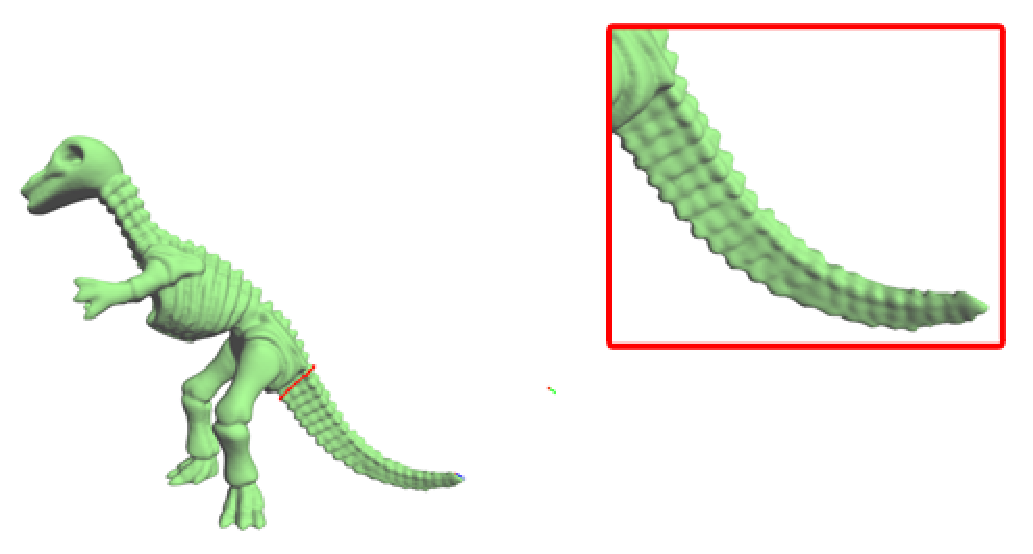
\includegraphics[scale=0.29]{figs/f5.5.original_pc-2.eps}
    \end{minipage}}
   \\
  \subfigure[]{
    \centering
    \label{fig:deformdino:b}
    \begin{minipage}[b]{0.32\textwidth}
      \centering
      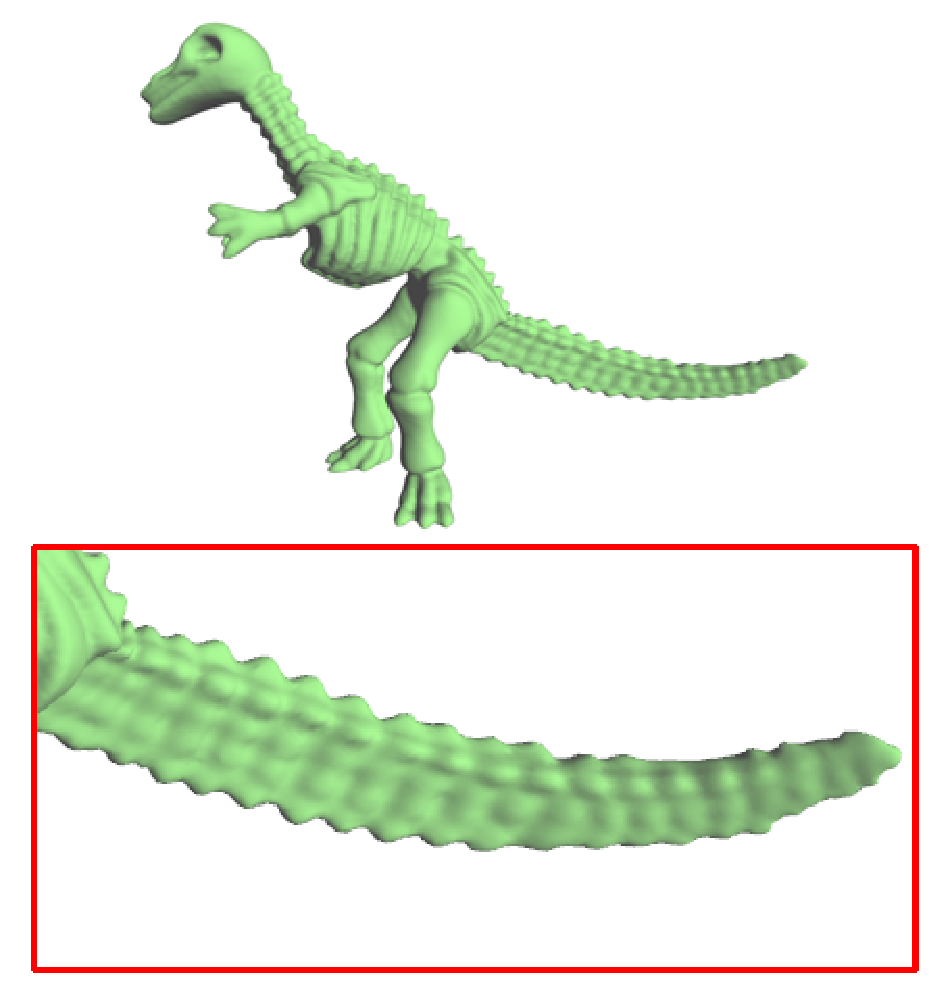
\includegraphics[scale=0.29]{figs/f5.5.ver0-3.eps}
    \end{minipage}}
  \subfigure[]{
    \centering
    \label{fig:deformdino:c}
    \begin{minipage}[b]{0.32\textwidth}
      \centering
      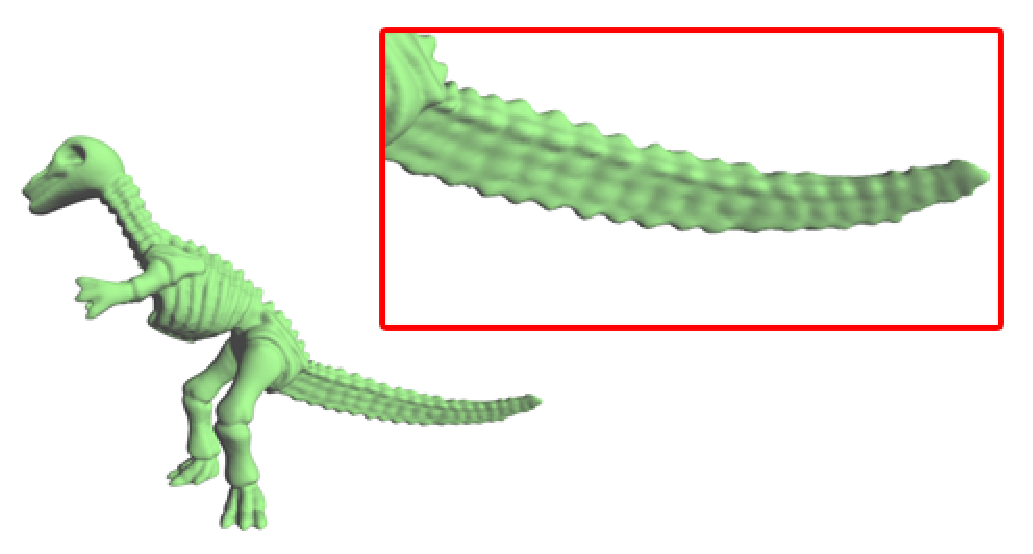
\includegraphics[scale=0.29]{figs/f5.5.ver05-3.eps}
    \end{minipage}}
  \subfigure[]{
    \centering
    \label{fig:deformdino:d}
    \begin{minipage}[b]{0.32\textwidth}
      \centering
      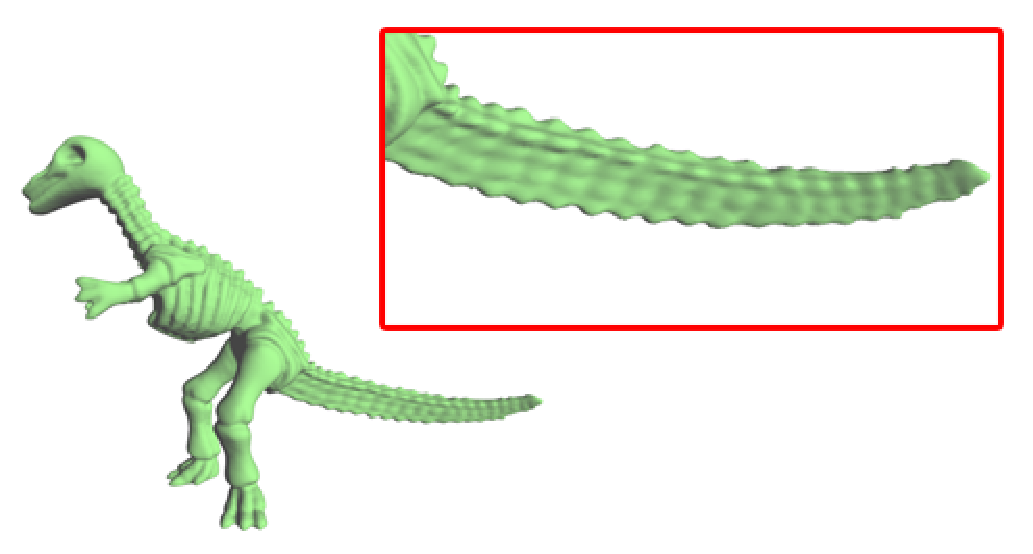
\includegraphics[scale=0.29]{figs/f5.5.ver10-3.eps}
    \end{minipage}}
  \\
  \subfigure[]{
    \centering
    \label{fig:deformdino:e} %% label for first subfigure
    \begin{minipage}[b]{0.32\textwidth}
      \centering
      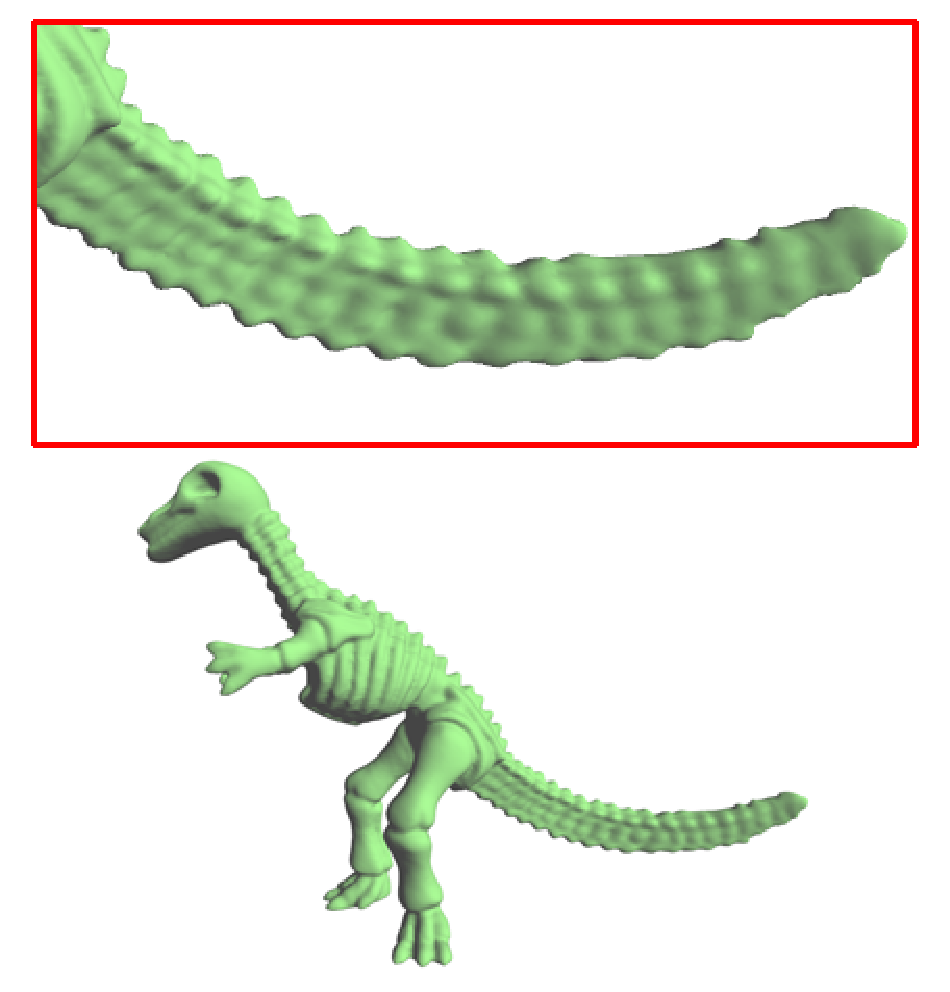
\includegraphics[scale=0.29]{figs/f5.5.edge0-3.eps}
    \end{minipage}}
  \subfigure[]{
    \centering
    \label{fig:deformdino:f}
    \begin{minipage}[b]{0.32\textwidth}
      \centering
      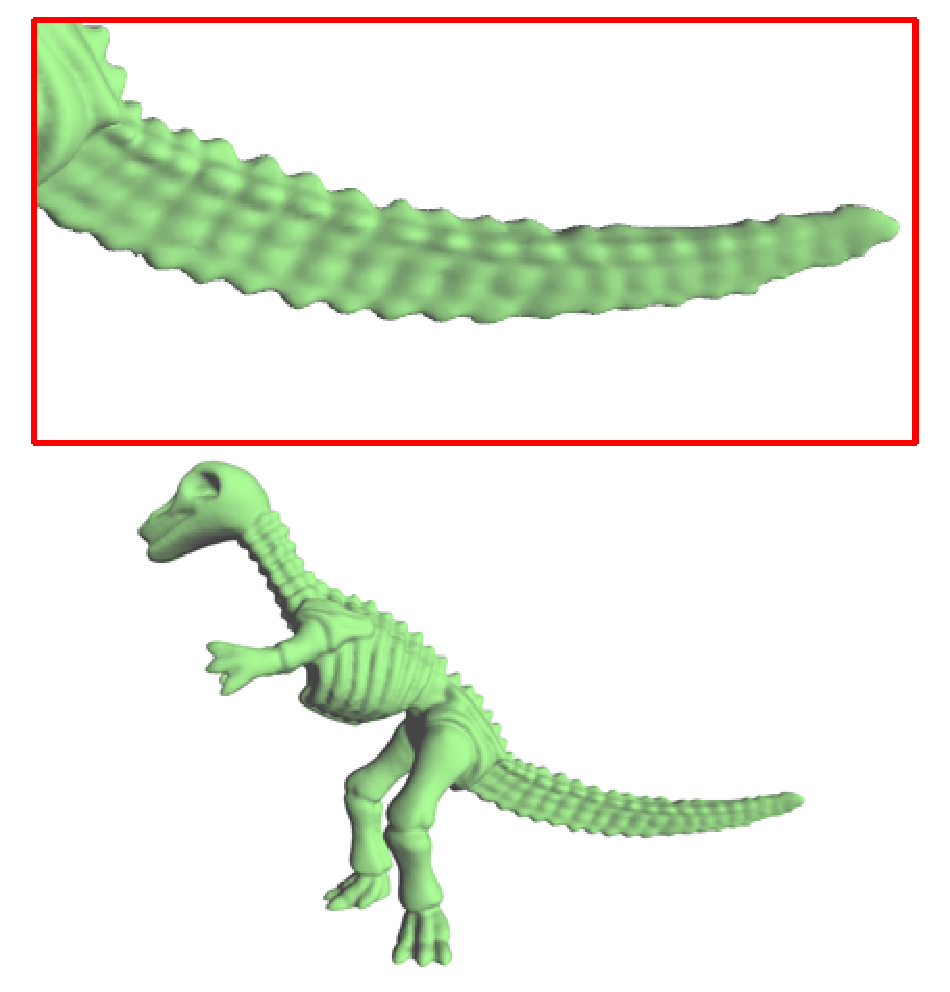
\includegraphics[scale=0.29]{figs/f5.5.edge05-3.eps}
    \end{minipage}}
  \subfigure[]{
    \centering
    \label{fig:deformdino:g}
    \begin{minipage}[b]{0.32\textwidth}
      \centering
      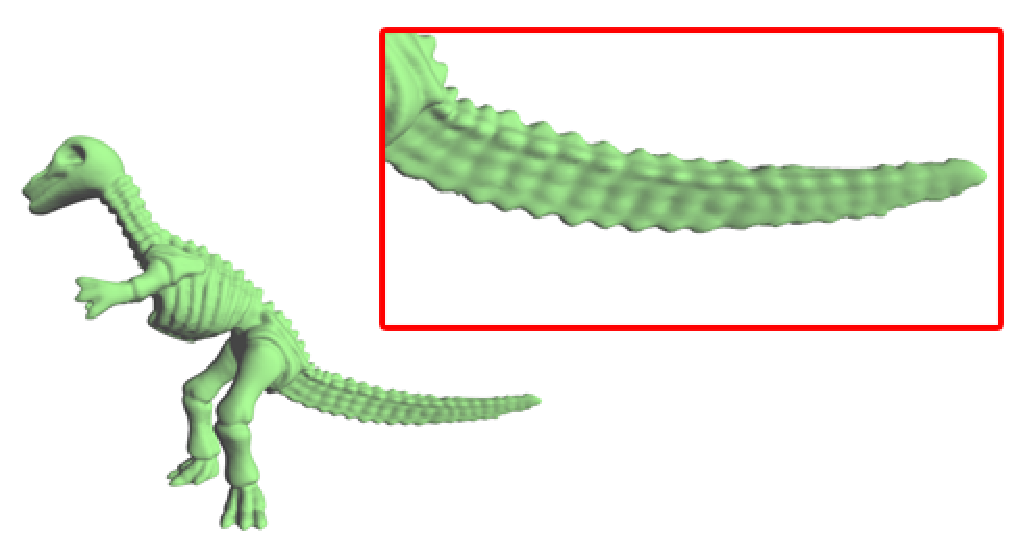
\includegraphics[scale=0.29]{figs/f5.5.edge10-3.eps}
    \end{minipage}}
  \caption{Flexible deformation of the \textit{Dinosaur} model. (a) The initial model. (b)-(d) Results of flexible deformation algorithm performed on the primal domain, with the global balance parameters valued 0, 0.5 and 1.0 respectively. (e)-(g) Results of flexible deformation algorithm performed via the edge-based graph, with the global balance parameters valued 0, 0.5 and 1.0 respectively. }
  \label{fig:deformdino} %% label for entire figure
\end{figure}

Here we provide sketching  tools, which are intuitive and flexible
for interactive designs, for the user to designate materials on
different parts of the mesh surface. The user can first set a scalar
value which represents the stiffness property of the material and
then use lasso or painting brush tools to specify the material for
the selected part. Since the entire user operations are performed on
the surface of the primal mesh while the calculations are implicitly
implemented on the edge-based graph, after the materials of the
primal vertices are specified, we calculate the material for each
node $\tilde{v_i}$ of the edge-based graph by averaging those of the
two end vertices of the primal edge $e_{ij}$ that $\tilde{v_i}$ lies
on.


\begin{figure} [htbp]
  \centering
  \subfigure[]{
    \centering
    \label{fig:deformbuf:a} %% label for first subfigure
    \begin{minipage}[b]{0.32\textwidth}
      \centering
      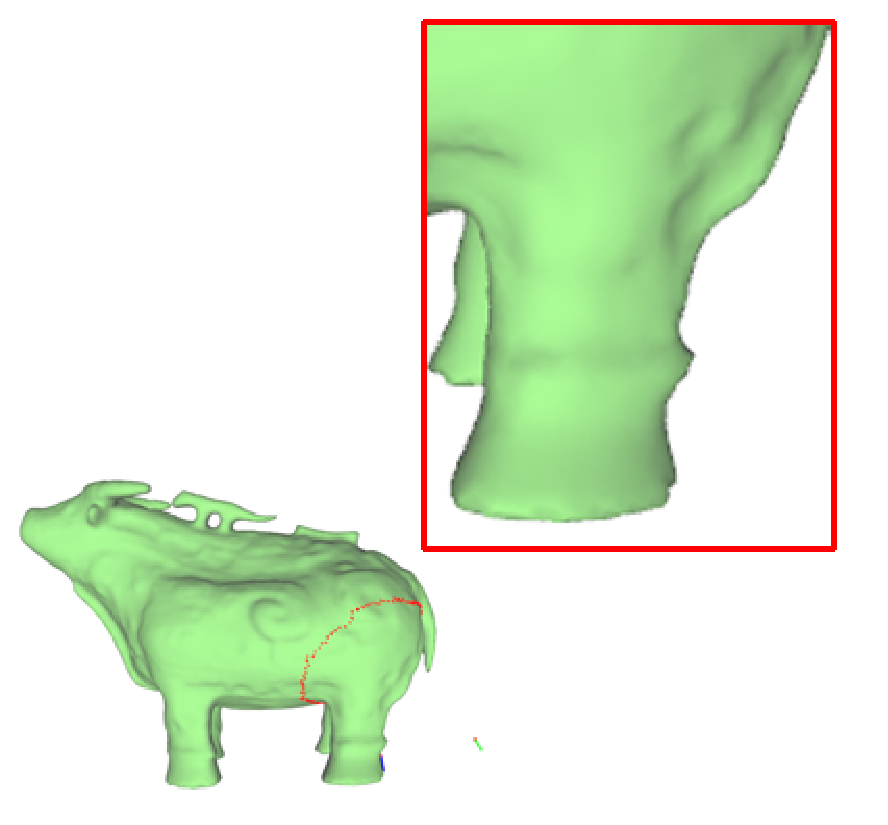
\includegraphics[scale=0.32]{figs/f5.6.original-pc-1.eps}
    \end{minipage}}
  \subfigure[]{
    \centering
    \label{fig:deformbuf:b}
    \begin{minipage}[b]{0.32\textwidth}
      \centering
      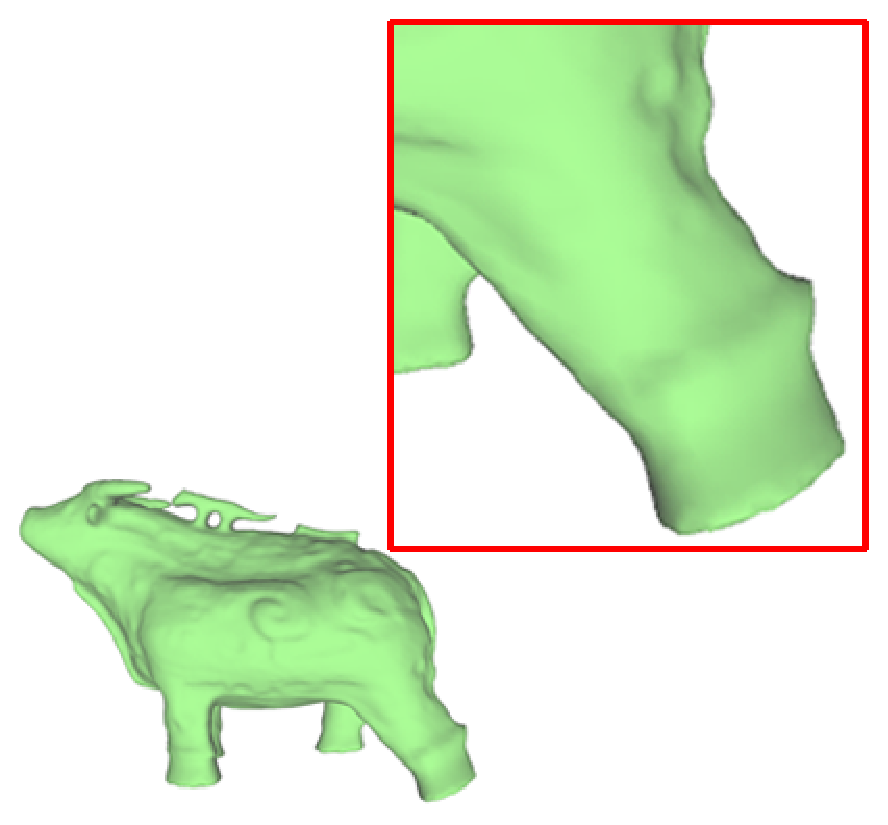
\includegraphics[scale=0.32]{figs/f5.6.0flexible-3.eps}
    \end{minipage}}
  \subfigure[]{
    \centering
    \label{fig:deformbuf:c}
    \begin{minipage}[b]{0.32\textwidth}
      \centering
      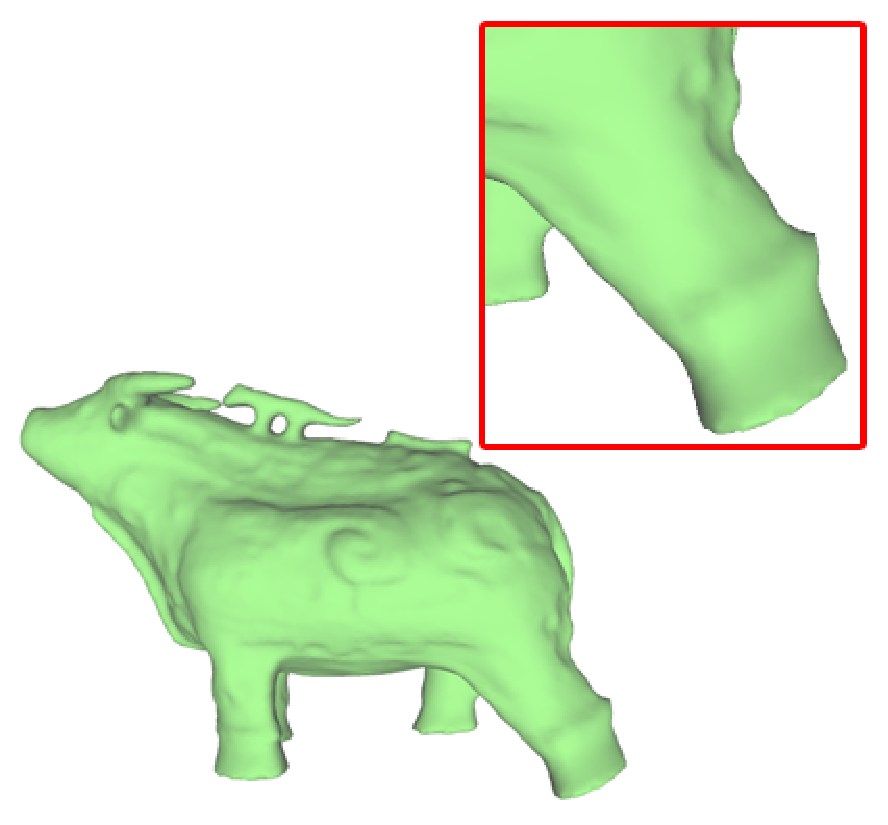
\includegraphics[scale=0.32]{figs/f5.6.2flexible-3.eps}
    \end{minipage}}
  \\
  \subfigure[]{
    \centering
    \label{fig:deformbuf:d}
    \begin{minipage}[b]{0.32\textwidth}
      \centering
      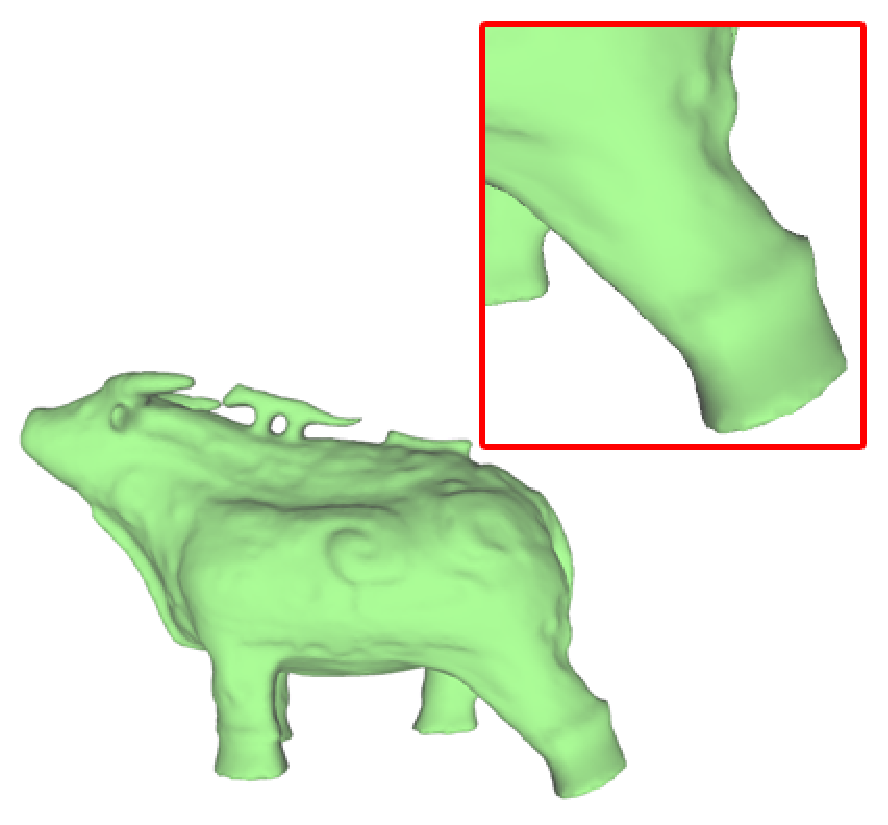
\includegraphics[scale=0.32]{figs/f5.6.5flexible-3.eps}
    \end{minipage}}
  \subfigure[]{
    \centering
    \label{fig:deformbuf:e} %% label for first subfigure
    \begin{minipage}[b]{0.32\textwidth}
      \centering
      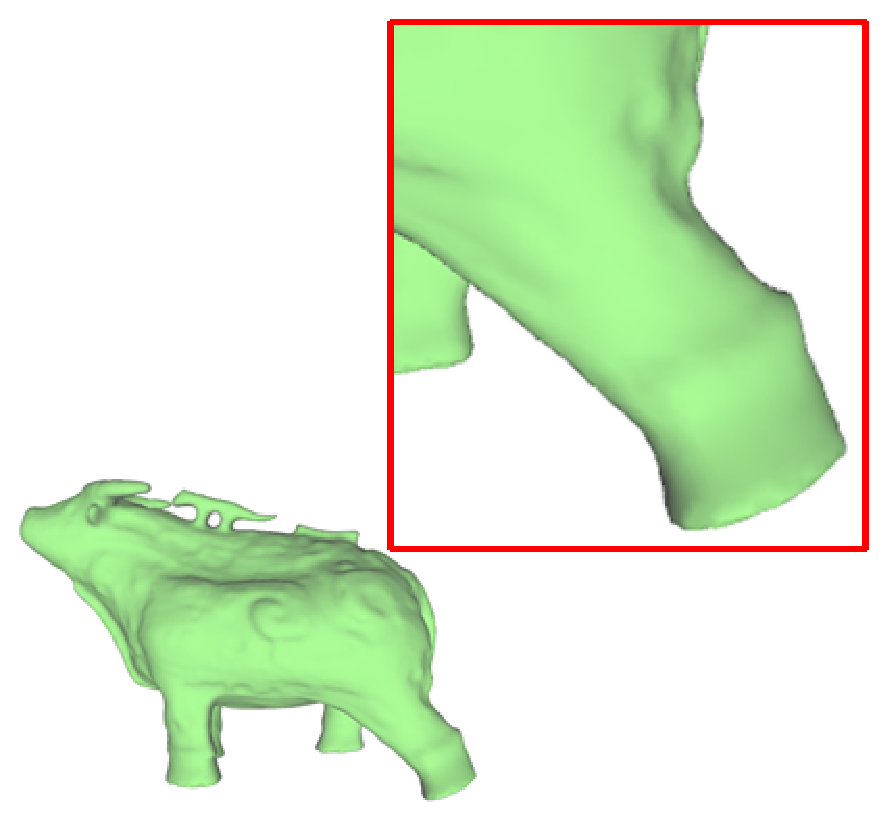
\includegraphics[scale=0.32]{figs/f5.6.8flexible-3.eps}
    \end{minipage}}
  \subfigure[]{
    \centering
    \label{fig:deformbuf:f}
    \begin{minipage}[b]{0.32\textwidth}
      \centering
      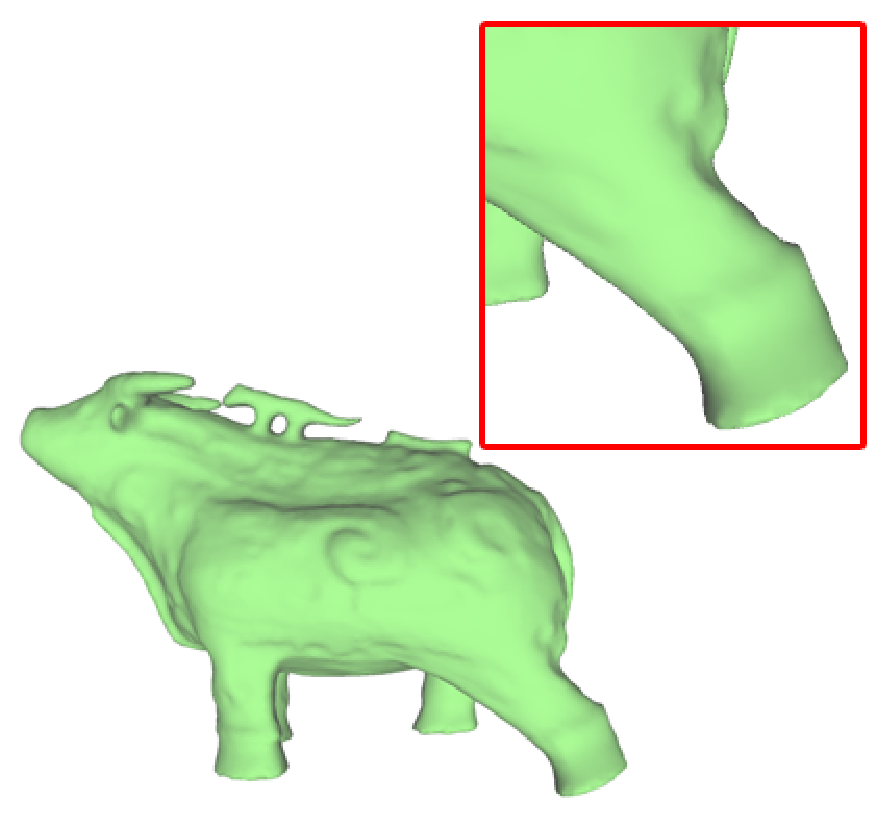
\includegraphics[scale=0.32]{figs/f5.6.10flexible-3.eps}
    \end{minipage}}
  \caption{Flexible deformation of the \textit{Buffle} model via the edge-based graph under different balance parameter values. (a) The initial model. (b)-(f) Deformation results with the global balance parameters valued 0, 0.2, 0.5, 0.8, 1.0 respectively. }
  \label{fig:deformbuf} %% label for entire figure
\end{figure}

\begin{figure} [htbp]
  \centering
  \subfigure[]{
    \centering
    \label{fig:deformJCglb:a} %% label for first subfigure
    \begin{minipage}[b]{0.32\textwidth}
      \centering
      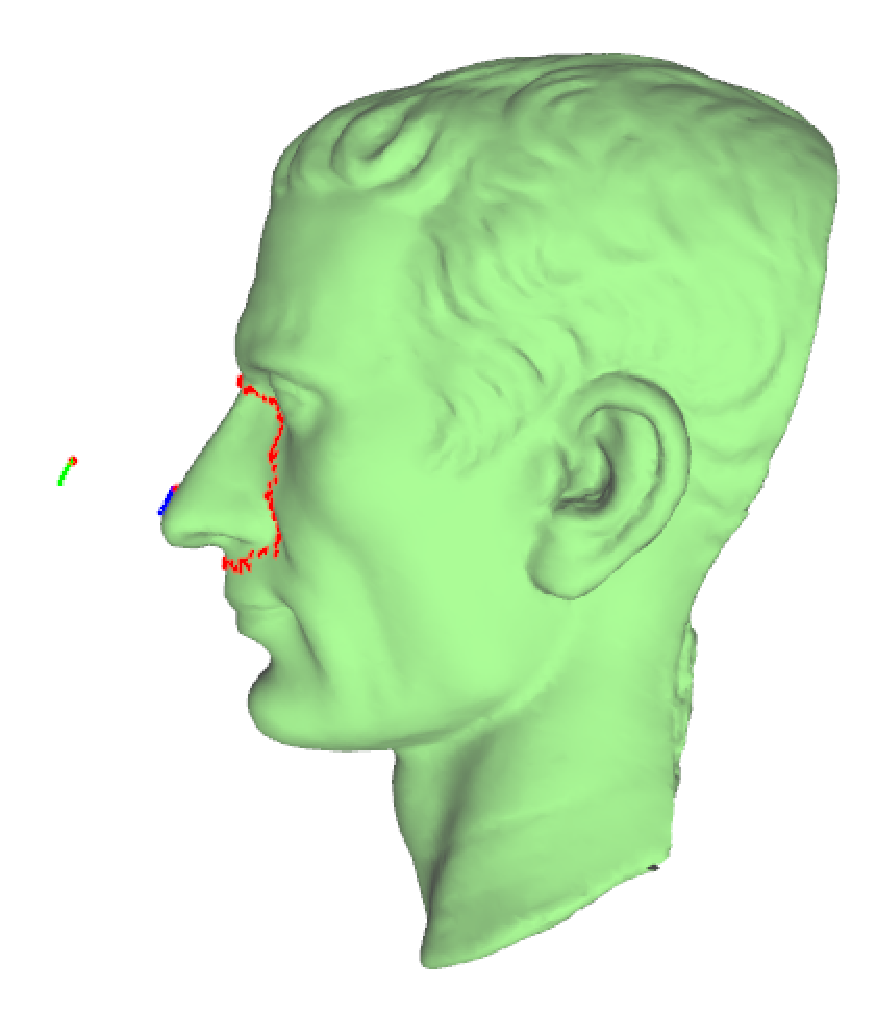
\includegraphics[scale=0.25]{figs/f5.7.julius--Caesar-pc-1.eps}
    \end{minipage}}
  \subfigure[]{
    \centering
    \label{fig:deformJCglb:b}
    \begin{minipage}[b]{0.32\textwidth}
      \centering
      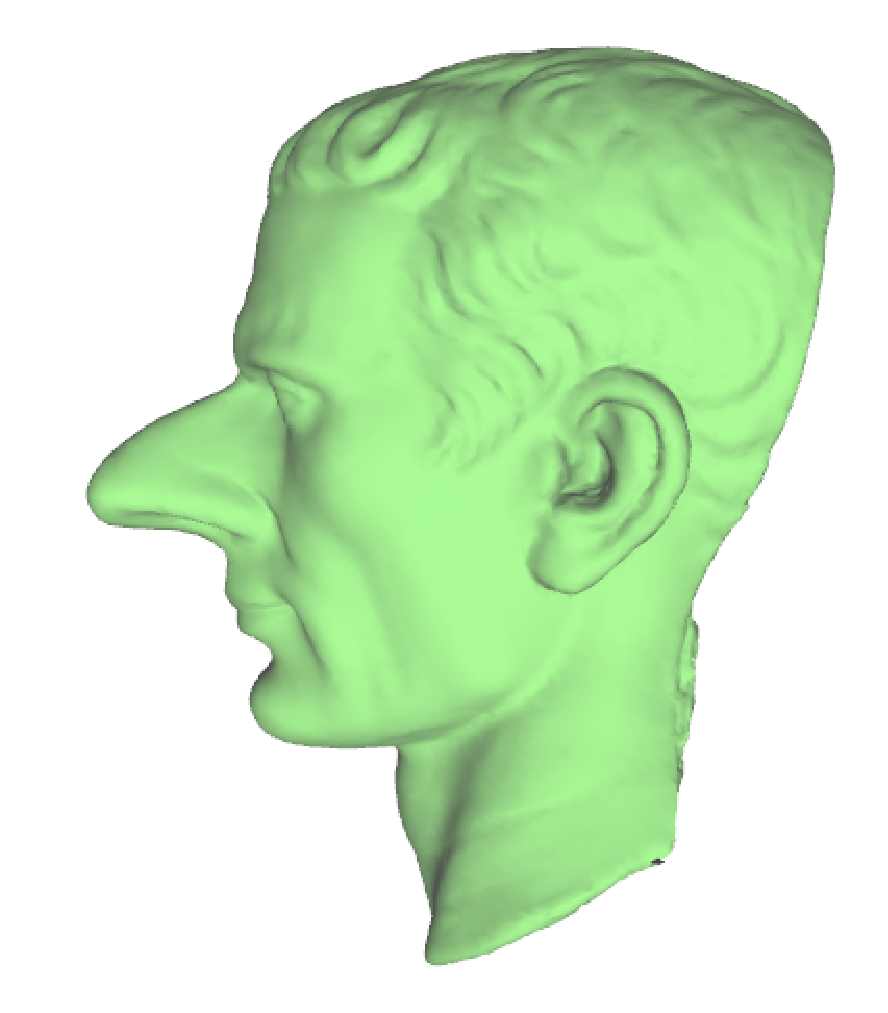
\includegraphics[scale=0.25]{figs/f5.7.0flexible-1.eps}
    \end{minipage}}
  \subfigure[]{
    \centering
    \label{fig:deformJCglb:c}
    \begin{minipage}[b]{0.32\textwidth}
      \centering
      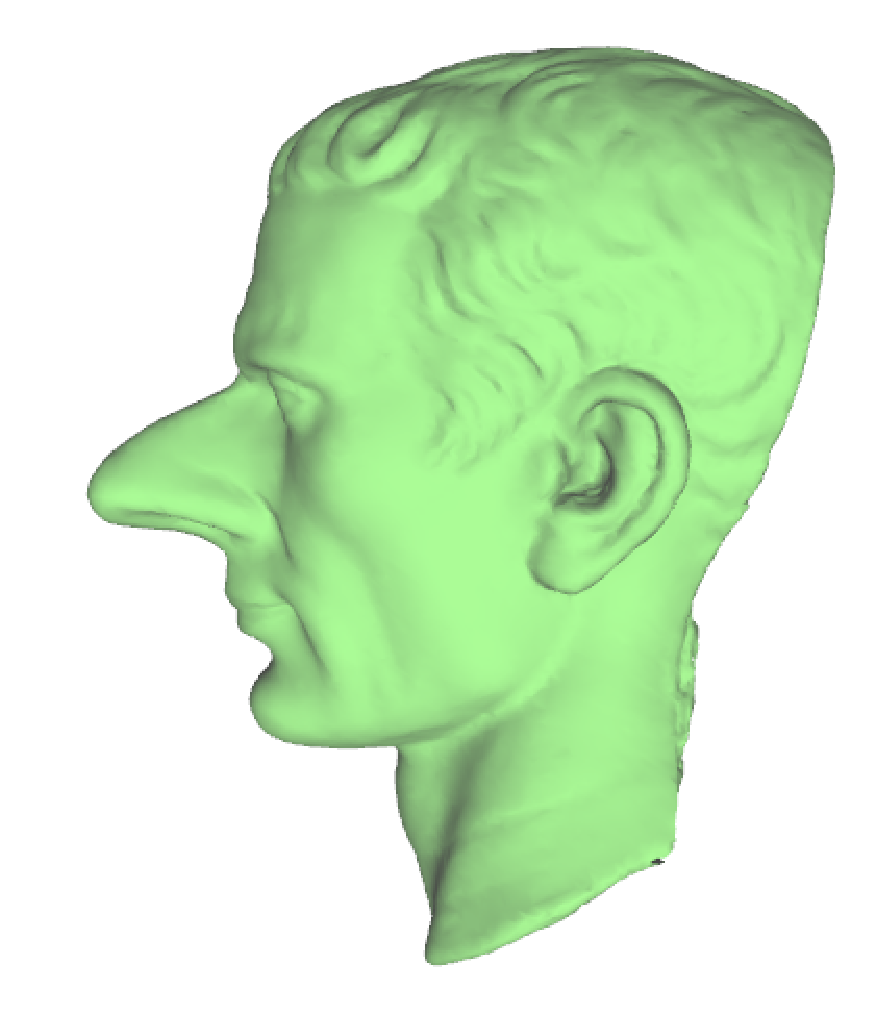
\includegraphics[scale=0.25]{figs/f5.7.2flexible-1.eps}
    \end{minipage}}
  \\
  \subfigure[]{
    \centering
    \label{fig:deformJCglb:d}
    \begin{minipage}[b]{0.32\textwidth}
      \centering
      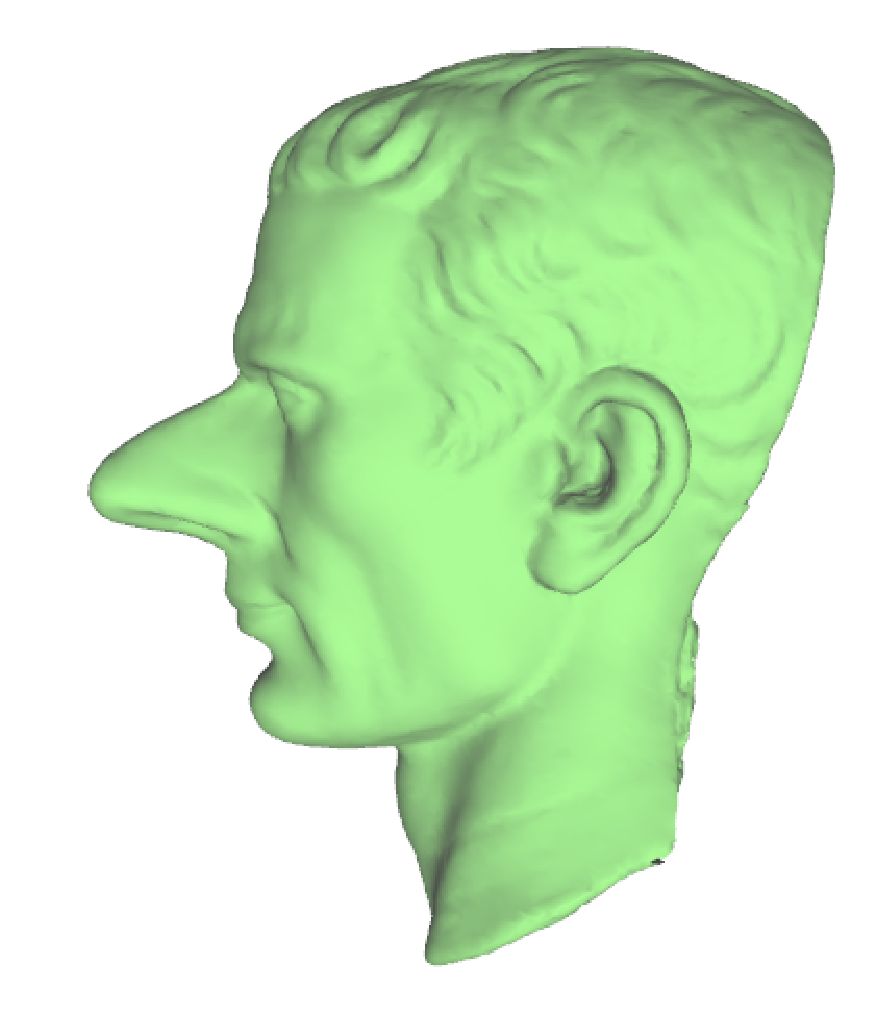
\includegraphics[scale=0.25]{figs/f5.7.5flexible-1.eps}
    \end{minipage}}
  \subfigure[]{
    \centering
    \label{fig:deformJCglb:e} %% label for first subfigure
    \begin{minipage}[b]{0.32\textwidth}
      \centering
      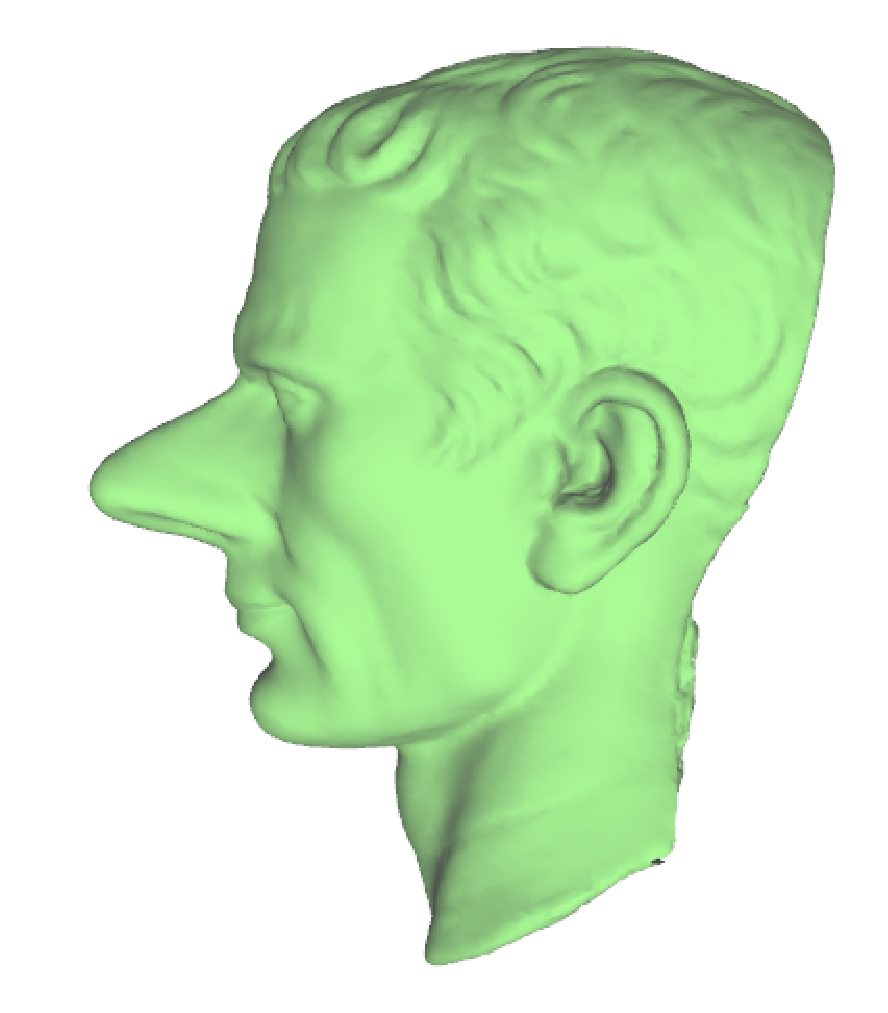
\includegraphics[scale=0.25]{figs/f5.7.8flexible-1.eps}
    \end{minipage}}
  \subfigure[]{
    \centering
    \label{fig:deformJCglb:f}
    \begin{minipage}[b]{0.32\textwidth}
      \centering
      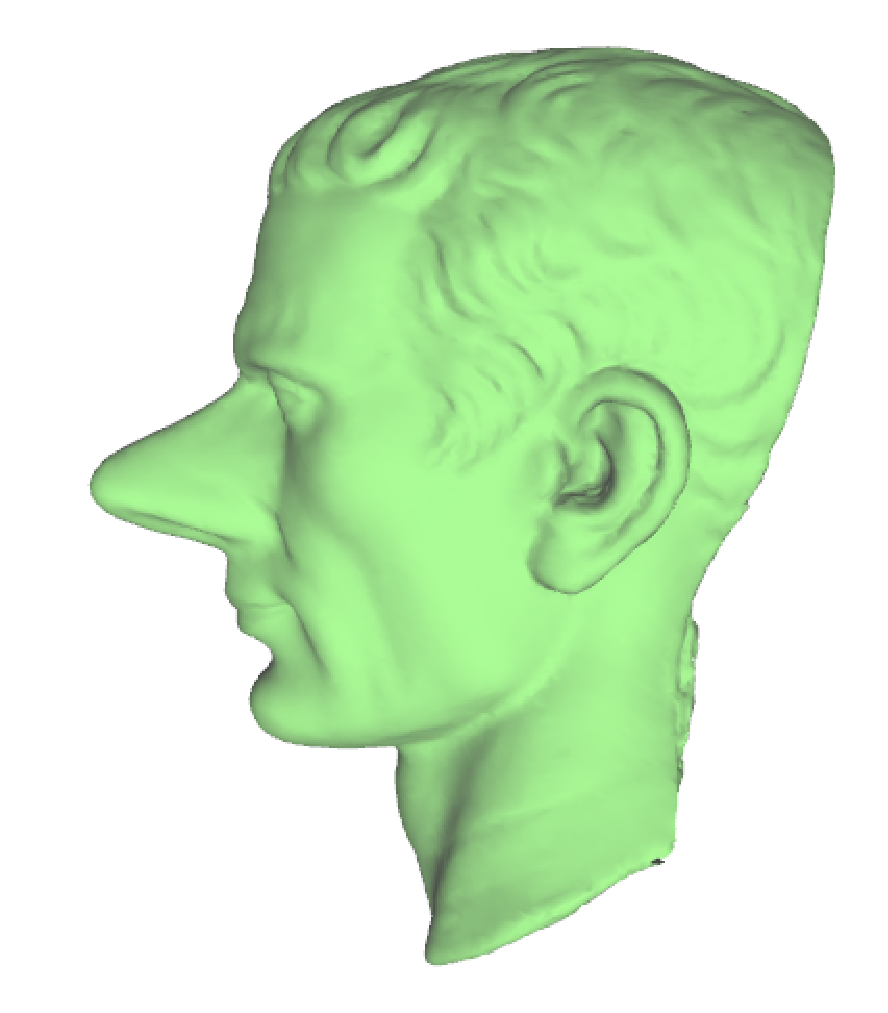
\includegraphics[scale=0.25]{figs/f5.7.10flexible-1.eps}
    \end{minipage}}
  \caption{Flexible deformation of the \textit{Julius-Caesar} model via the edge-based graph under different balance parameter values. (a) The initial model. (b)-(f) Deformation results with the global balance parameters valued 0, 0.2, 0.5, 0.8, 1.0 respectively. }
  \label{fig:deformJCglb} %% label for entire figure
\end{figure}


Results of the local method can be seen in Figures~\ref{fig:deformplane} to~\ref{fig:deformpig}.

\begin{figure} [htbp]
  \centering
  \subfigure[]{
    \centering
    \label{fig:deformplane:a} %% label for first subfigure
    \begin{minipage}[b]{0.7\textwidth}
      \centering
      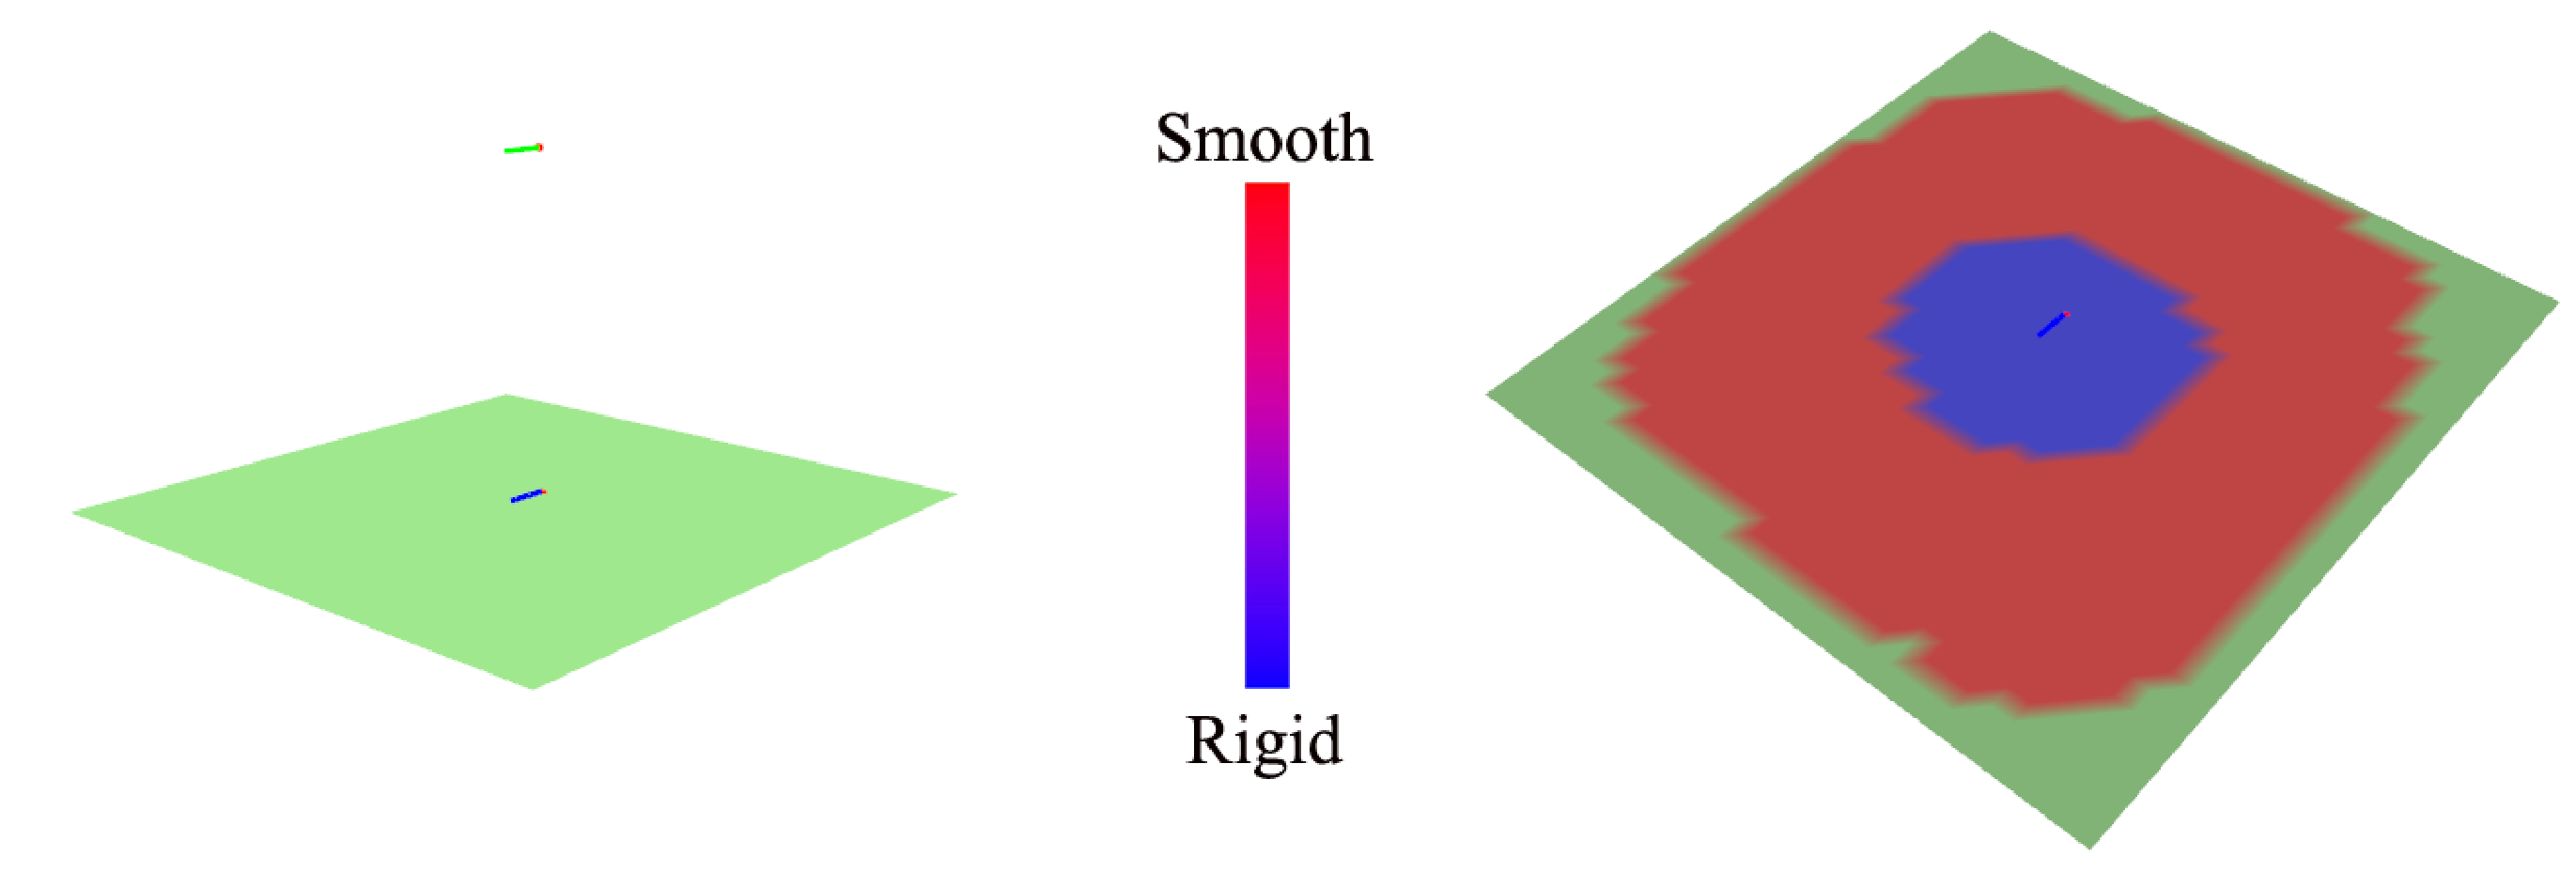
\includegraphics[scale=0.20]{figs/f5.8.planeMat2.eps}
    \end{minipage}}
  \\
  \subfigure[]{
    \centering
    \label{fig:deformplane:b}
    \begin{minipage}[b]{0.32\textwidth}
      \centering
      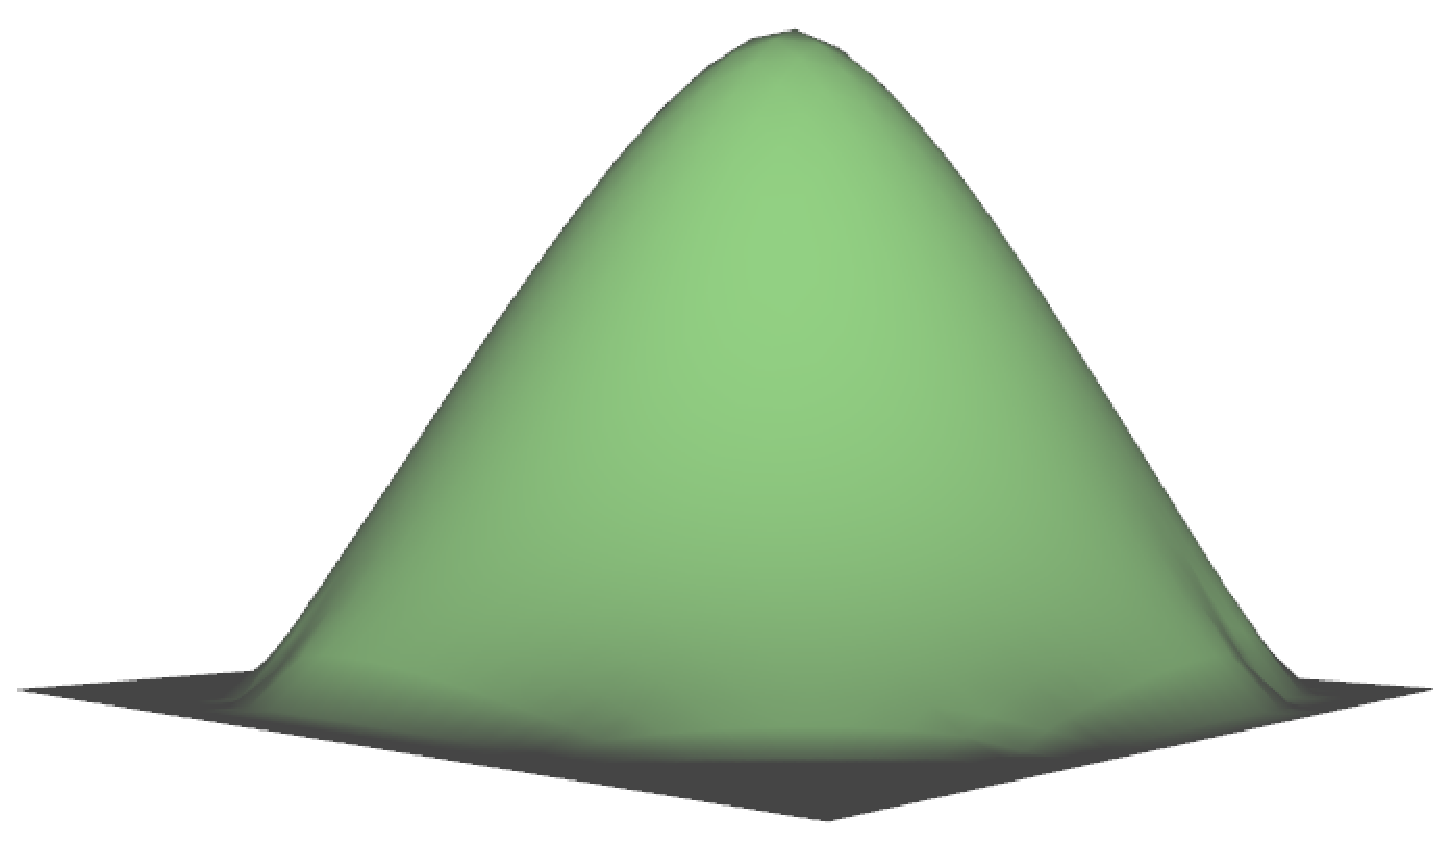
\includegraphics[scale=0.20]{figs/f5.8.ver0-iso-1.eps}
    \end{minipage}}
  \subfigure[]{
    \centering
    \label{fig:deformplane:c}
    \begin{minipage}[b]{0.32\textwidth}
      \centering
      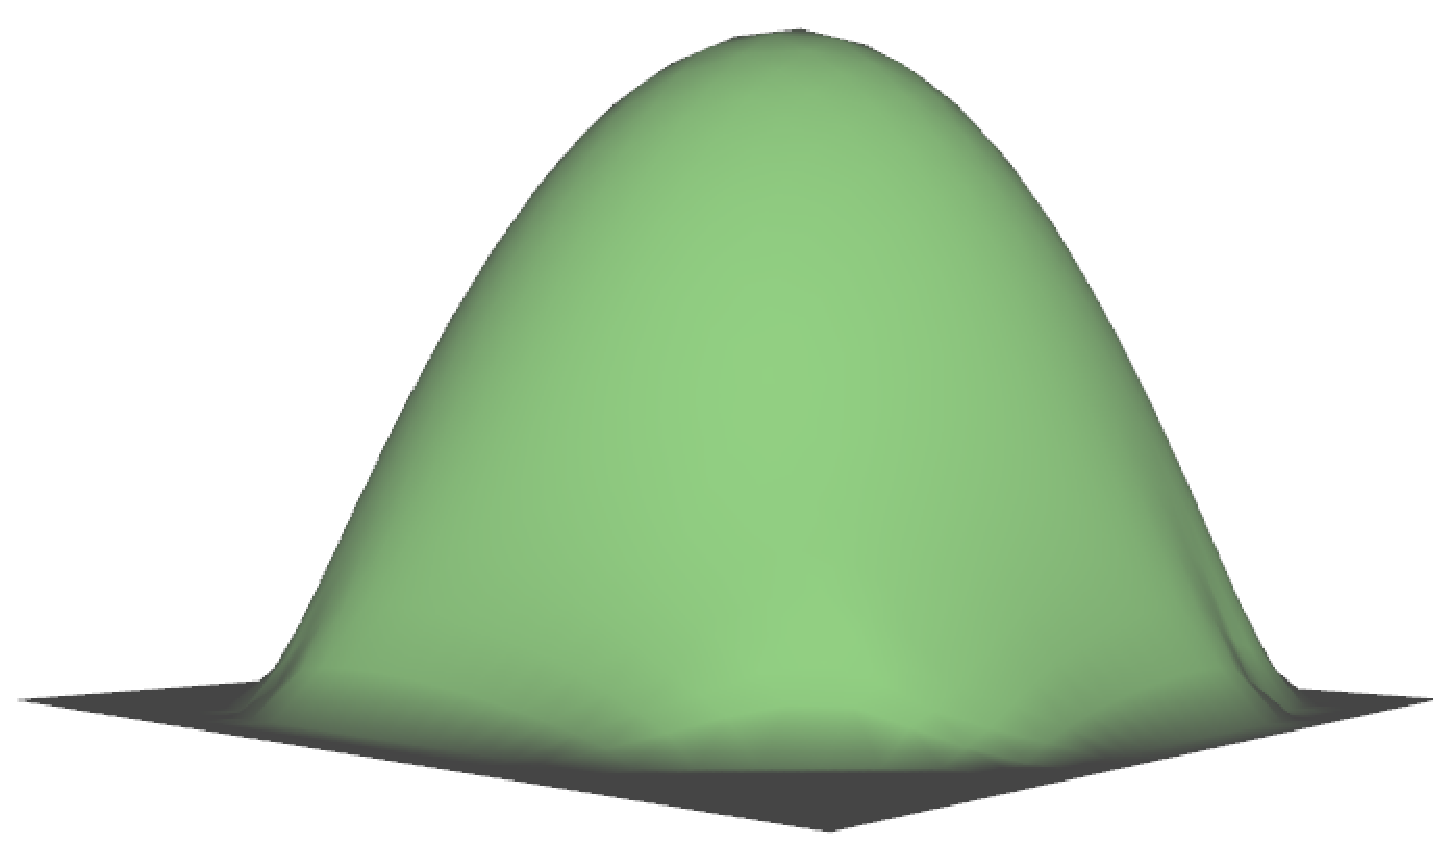
\includegraphics[scale=0.20]{figs/f5.8.ver10-iso-1.eps}
    \end{minipage}}
  \subfigure[]{
    \centering
    \label{fig:deformplane:d}
    \begin{minipage}[b]{0.32\textwidth}
      \centering
      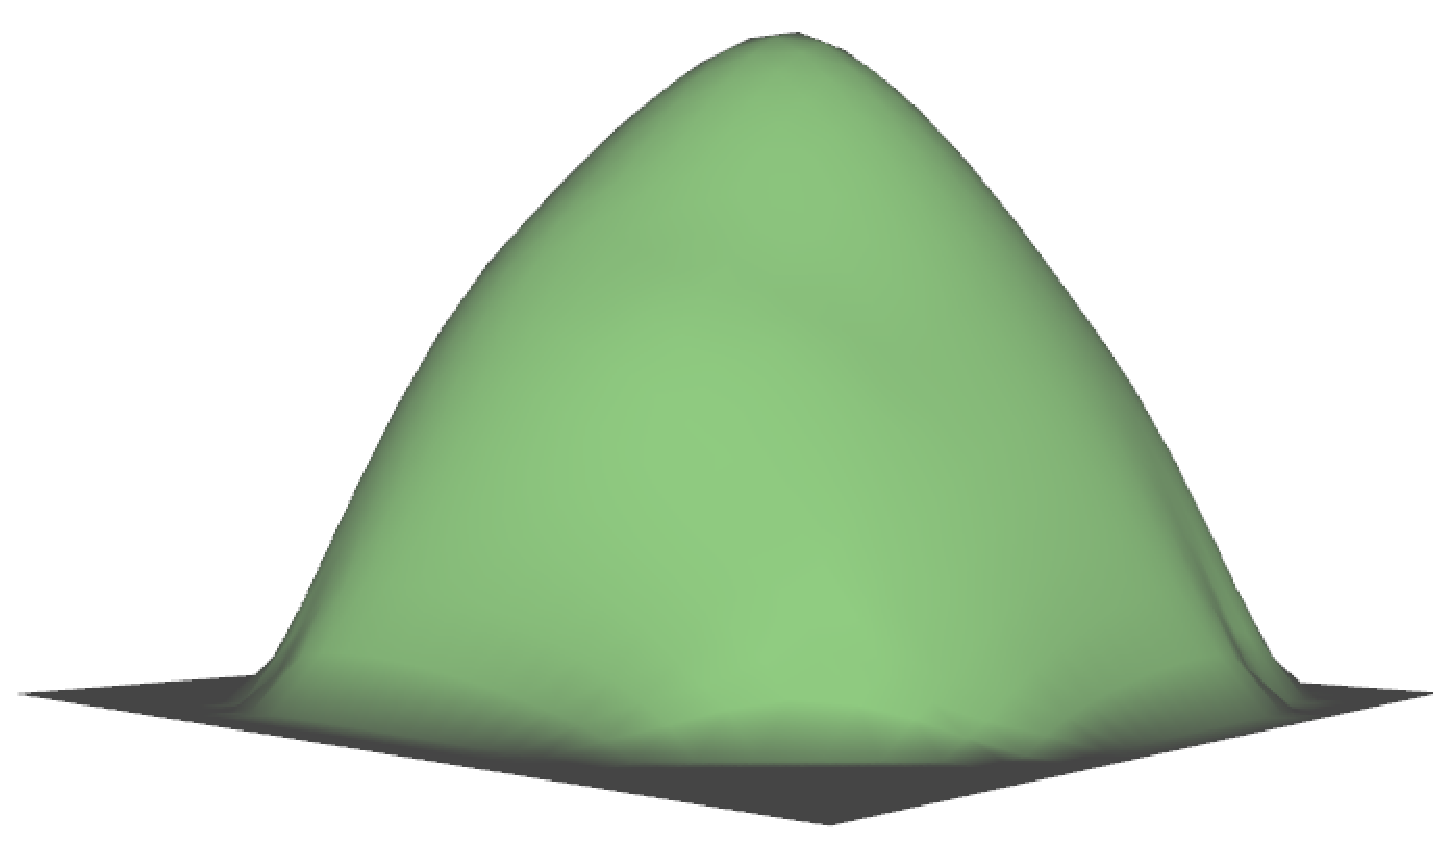
\includegraphics[scale=0.20]{figs/f5.8.verMat-iso-1.eps}
    \end{minipage}}
  \caption{Material-constrained deformation result of the \textit{plane} model. (a) The initial model and its specified materials. (b)-(c) Deformation results of uniformly distributed materials with global balance parameter valued 0 and 1 respectively. (d) Deformation result with the specified non-uniform materials.}
  \label{fig:deformplane} %% label for entire figure
\end{figure}

\begin{figure} [htbp]
  \centering
  \subfigure[]{
    \centering
    \label{fig:deformJCMat:a} %% label for first subfigure
    \begin{minipage}[b]{0.7\textwidth}
      \centering
      \includegraphics[scale=0.18]{figs/f5.9.JSMat2.eps}
    \end{minipage}}
  \\
  \subfigure[]{
    \centering
    \label{fig:deformJCMat:b}
    \begin{minipage}[b]{0.23\textwidth}
      \centering
      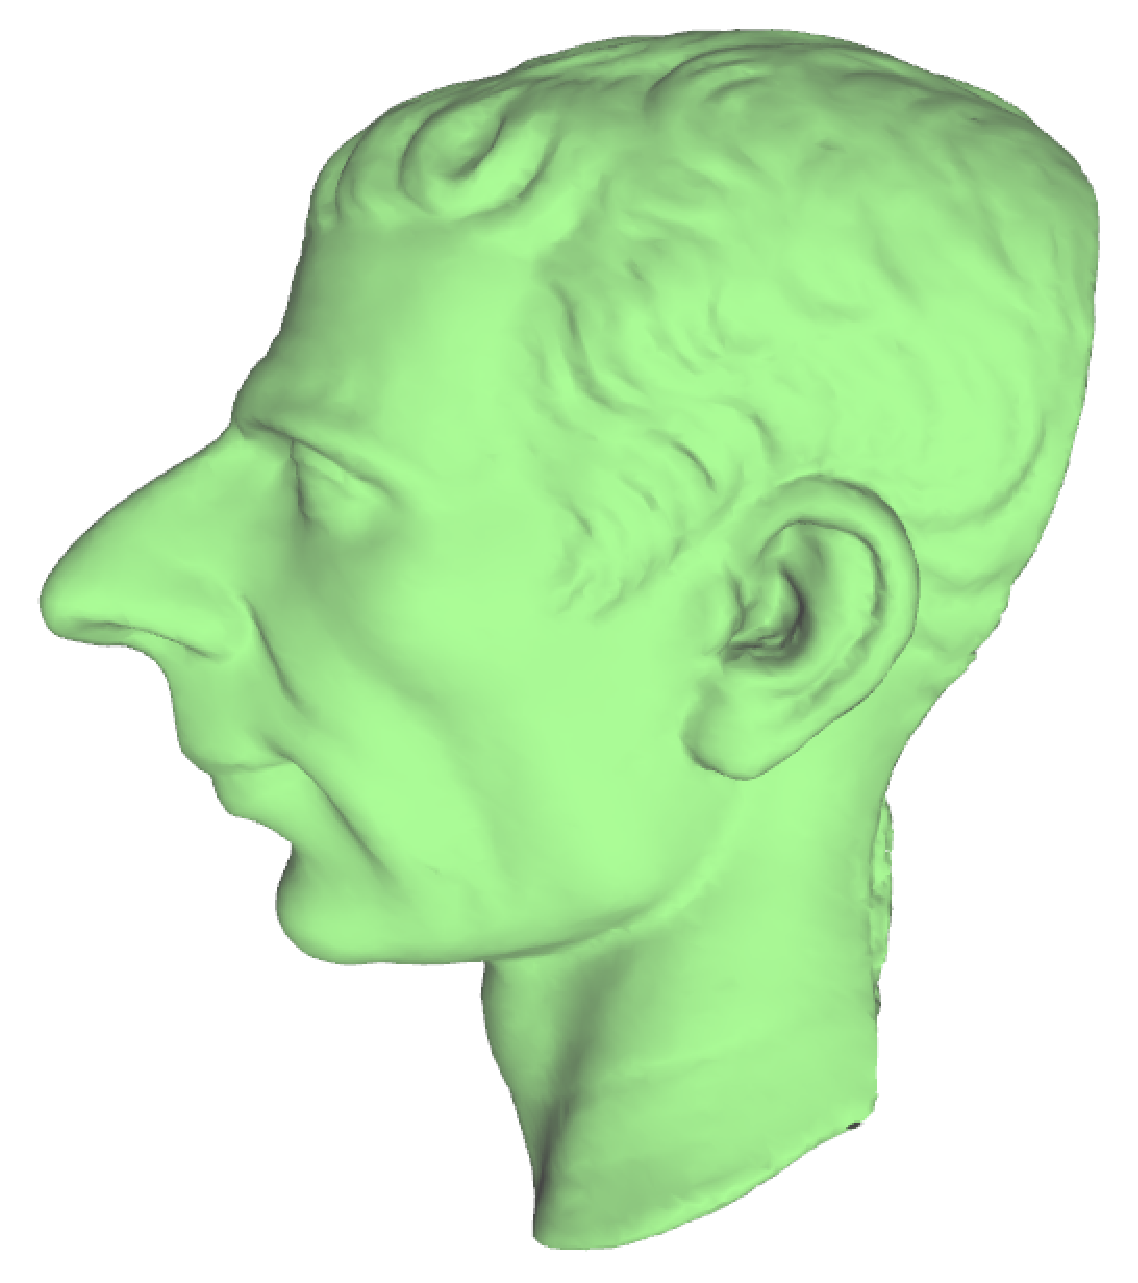
\includegraphics[scale=0.18]{figs/f5.9.ver0-iso-1.eps}
    \end{minipage}}
  \subfigure[]{
    \centering
    \label{fig:deformJCMat:c}
    \begin{minipage}[b]{0.23\textwidth}
      \centering
      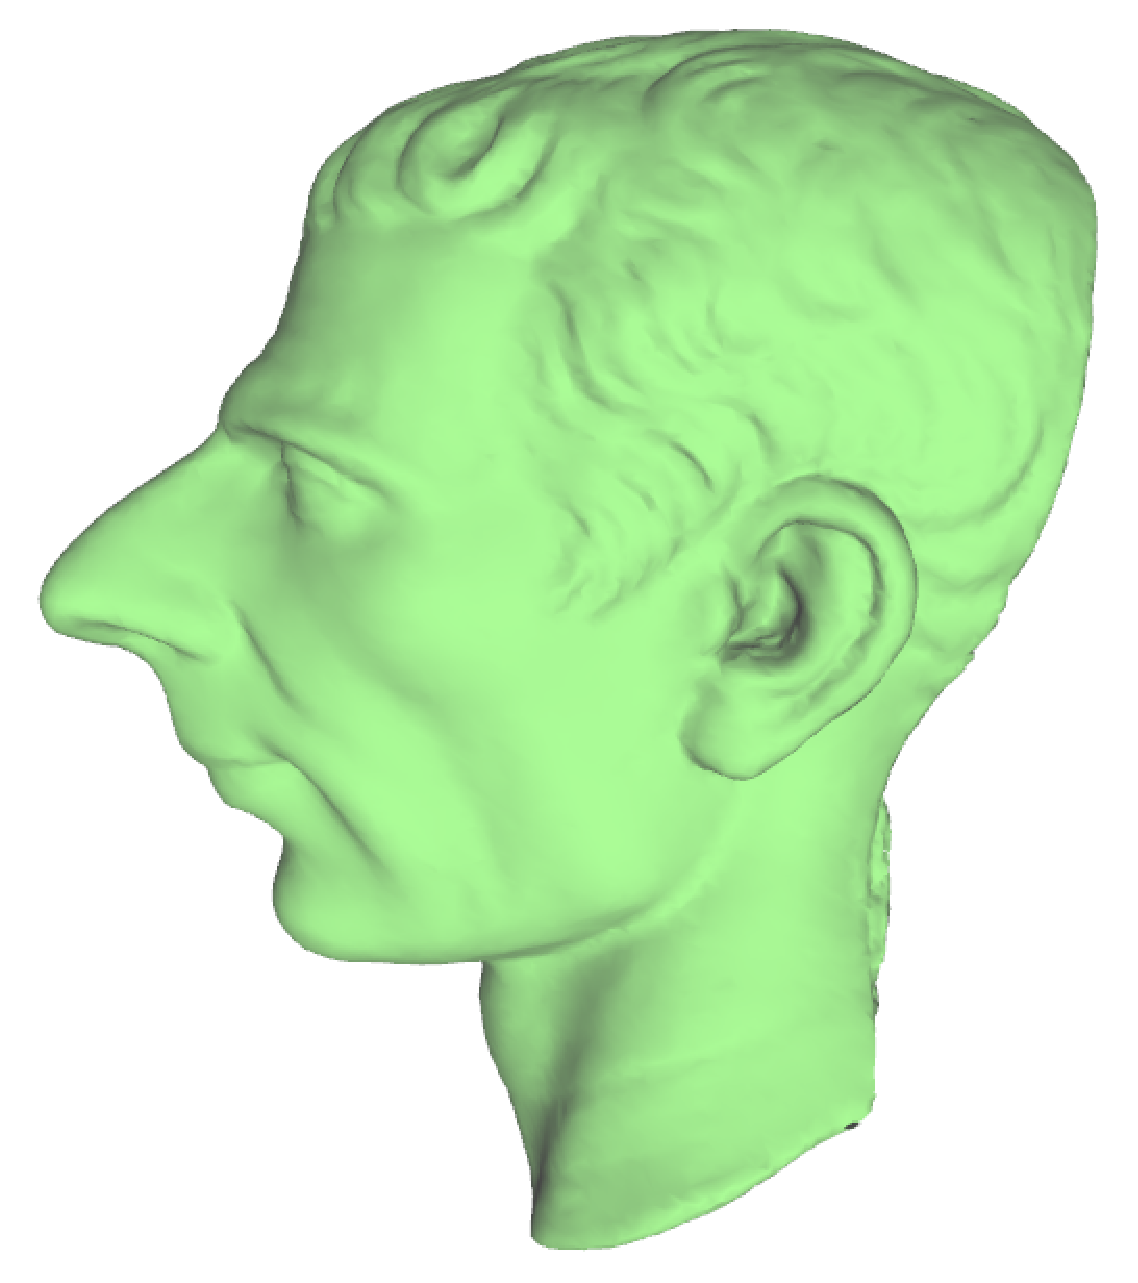
\includegraphics[scale=0.18]{figs/f5.9.ver05-iso-1.eps}
    \end{minipage}}
  \subfigure[]{
    \centering
    \label{fig:deformJCMat:d}
    \begin{minipage}[b]{0.23\textwidth}
      \centering
      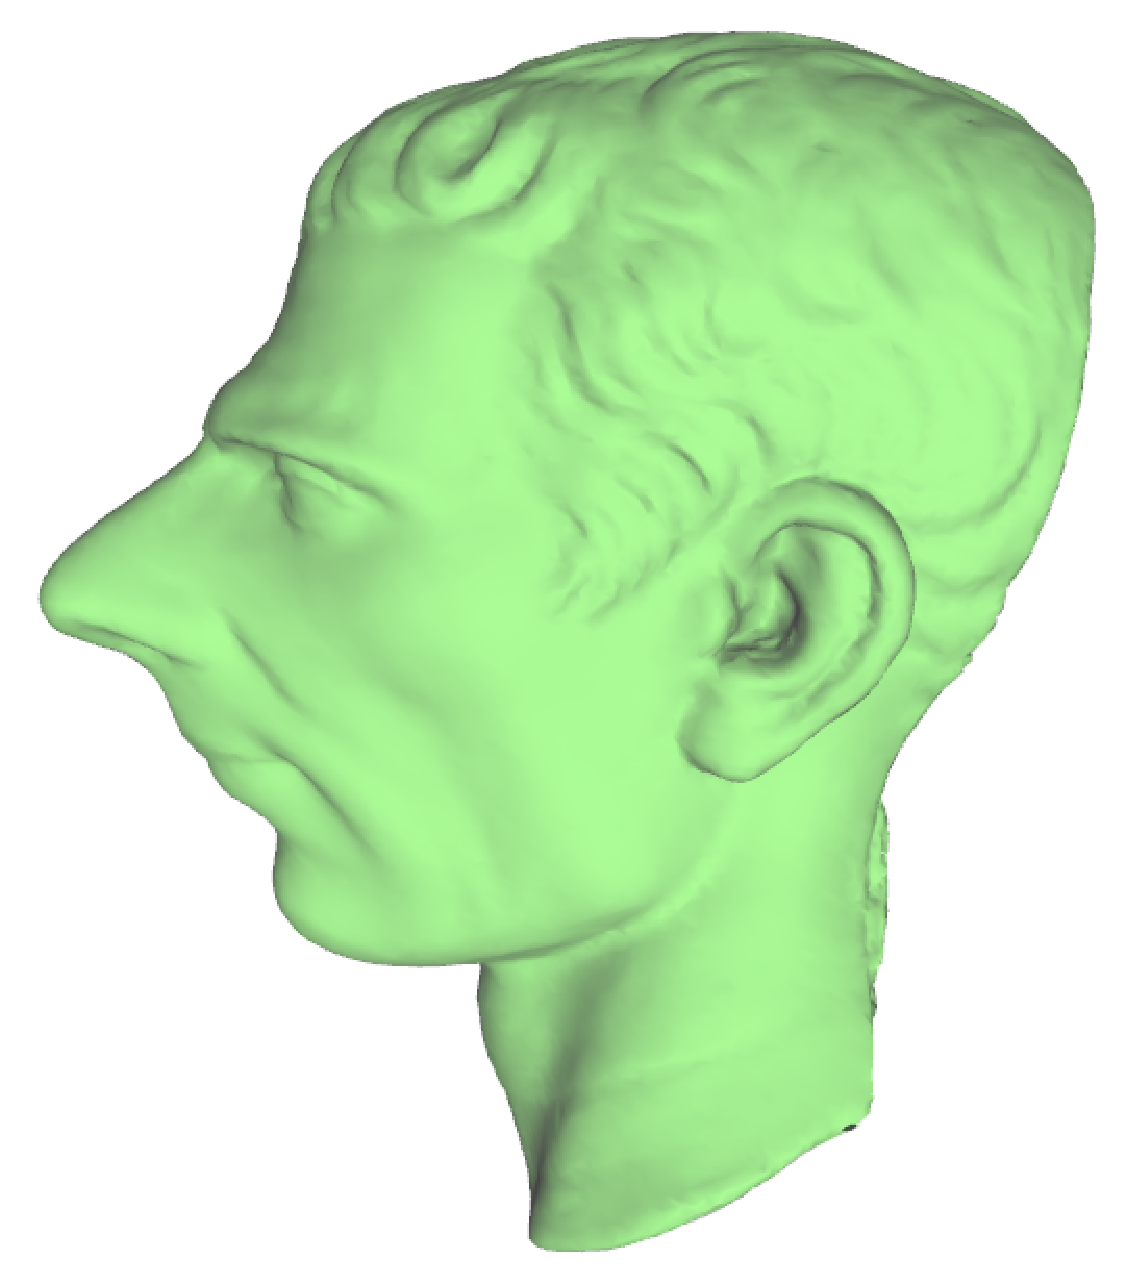
\includegraphics[scale=0.18]{figs/f5.9.ver10-iso-1.eps}
    \end{minipage}}
  \subfigure[]{
    \centering
    \label{fig:deformJCMat:e}
    \begin{minipage}[b]{0.23\textwidth}
      \centering
      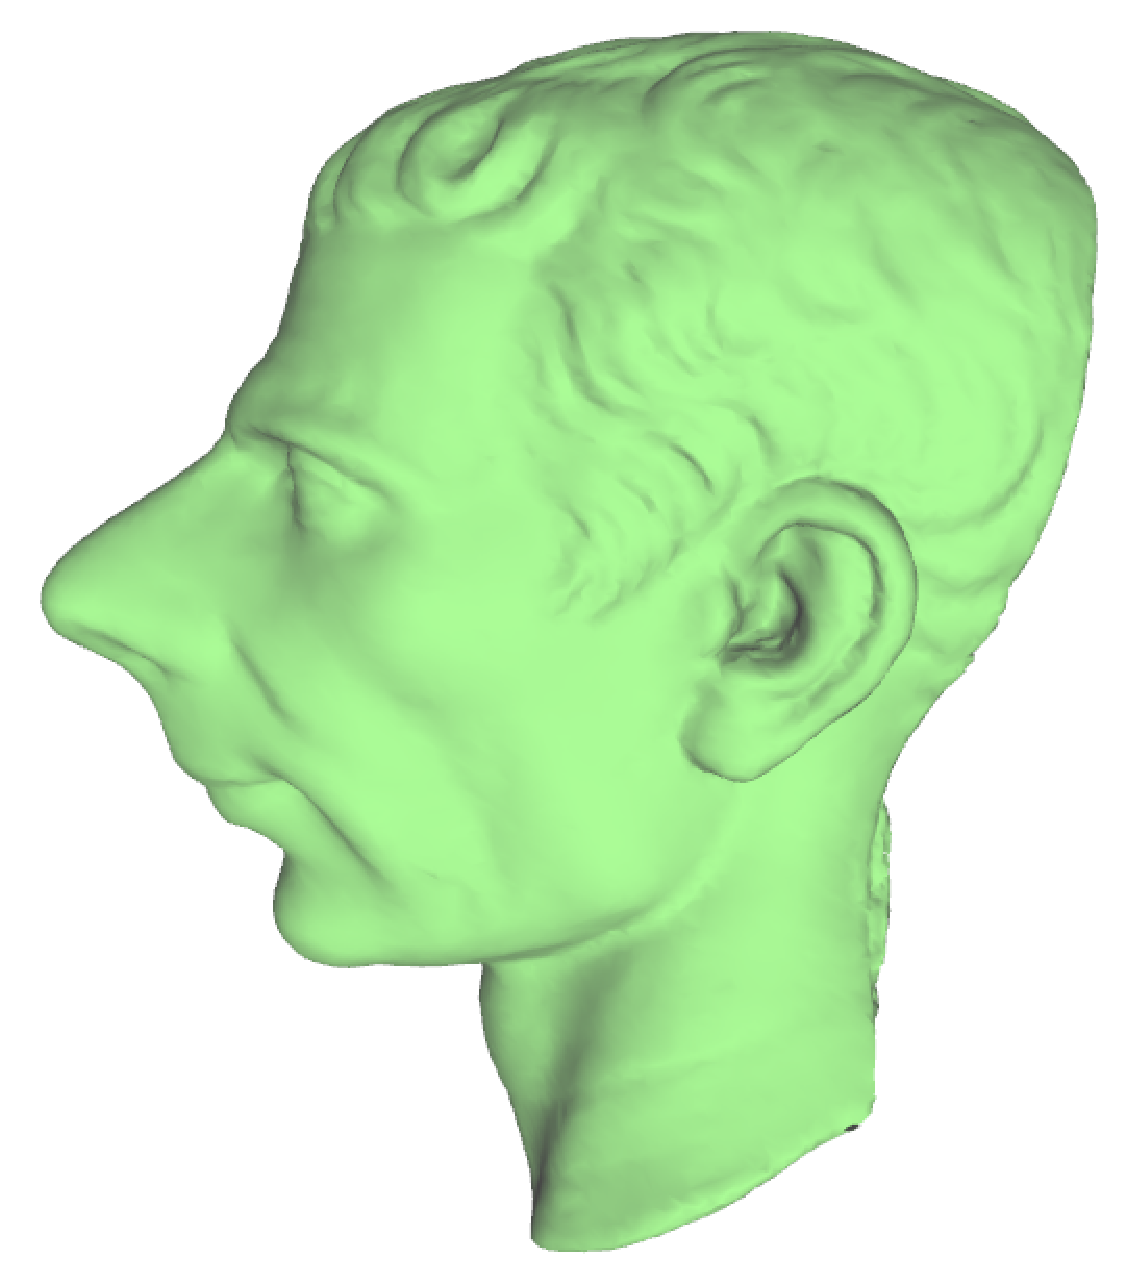
\includegraphics[scale=0.18]{figs/f5.9.verMat-iso-1.eps}
    \end{minipage}}
  \caption{Material-constrained deformation of the \textit{Julius-Caesar} model. (a) The initial model and its specified materials. (b)-(d) Deformation results of uniformly distributed materials with global balance parameter valued 0, 0.5 and 1 respectively. (e) Deformation result with the specified non-uniform materials.}
  \label{fig:deformJCMat} %% label for entire figure
\end{figure}

\begin{figure} [htbp]
  \centering
  \subfigure[]{
    \centering
    \label{fig:deformpig:a} %% label for first subfigure
    \begin{minipage}[b]{0.7\textwidth}
      \centering
      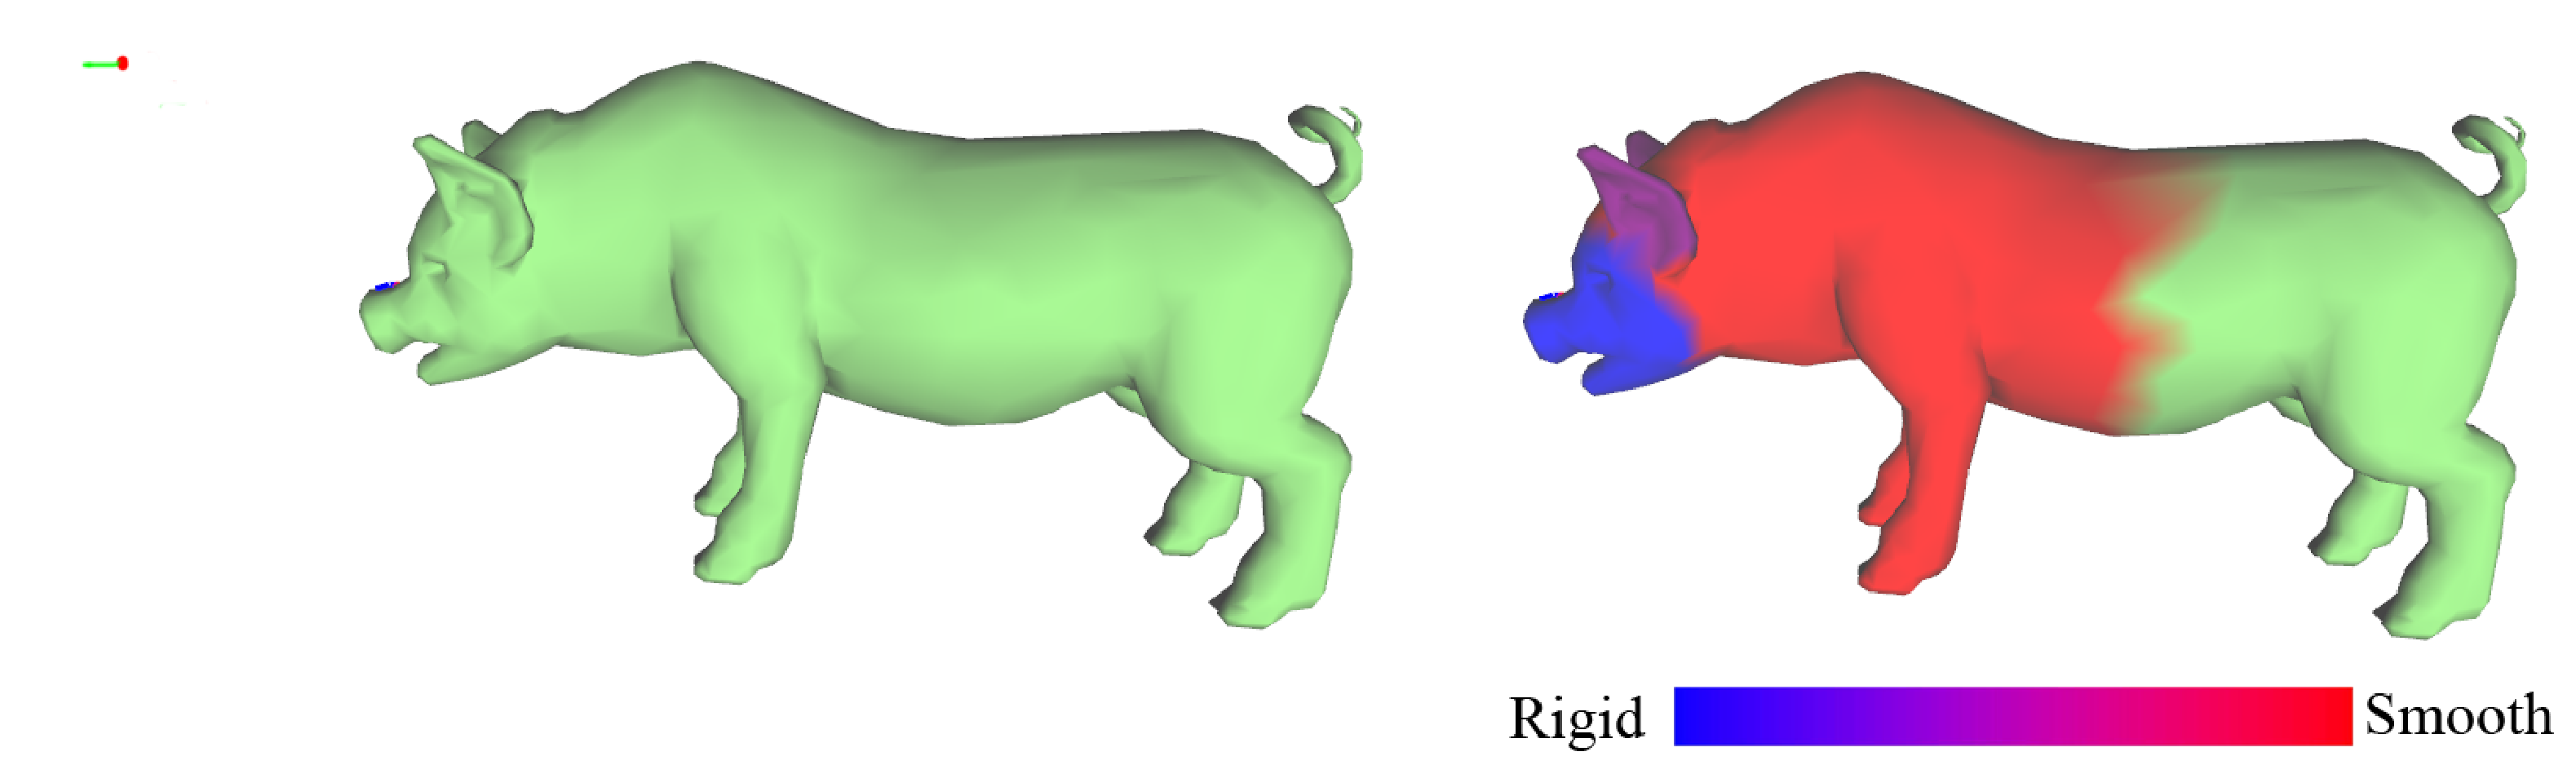
\includegraphics[scale=0.18]{figs/f5.10.PigMat1-with-curve.eps}
    \end{minipage}}
  \\
  \subfigure[]{
    \centering
    \label{fig:deformpig:b}
    \begin{minipage}[b]{0.23\textwidth}
      \centering
      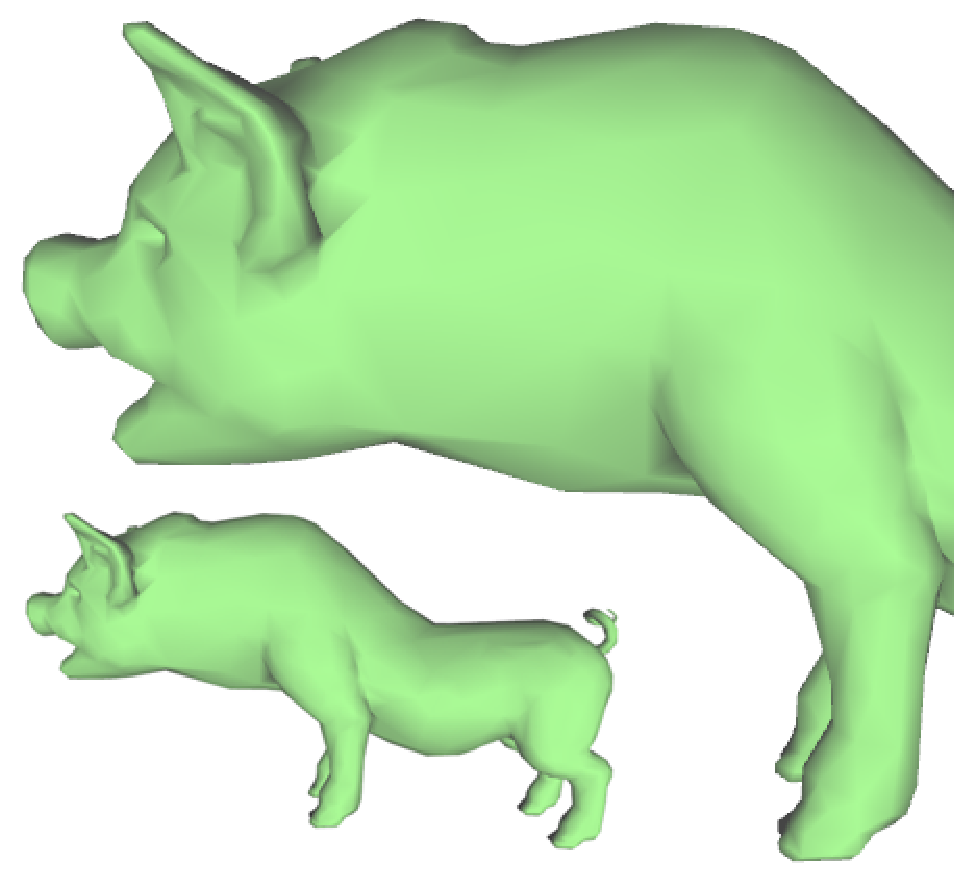
\includegraphics[scale=0.18]{figs/f5.10.PigMat2.eps}
    \end{minipage}}
  \subfigure[]{
    \centering
    \label{fig:deformpig:c}
    \begin{minipage}[b]{0.23\textwidth}
      \centering
      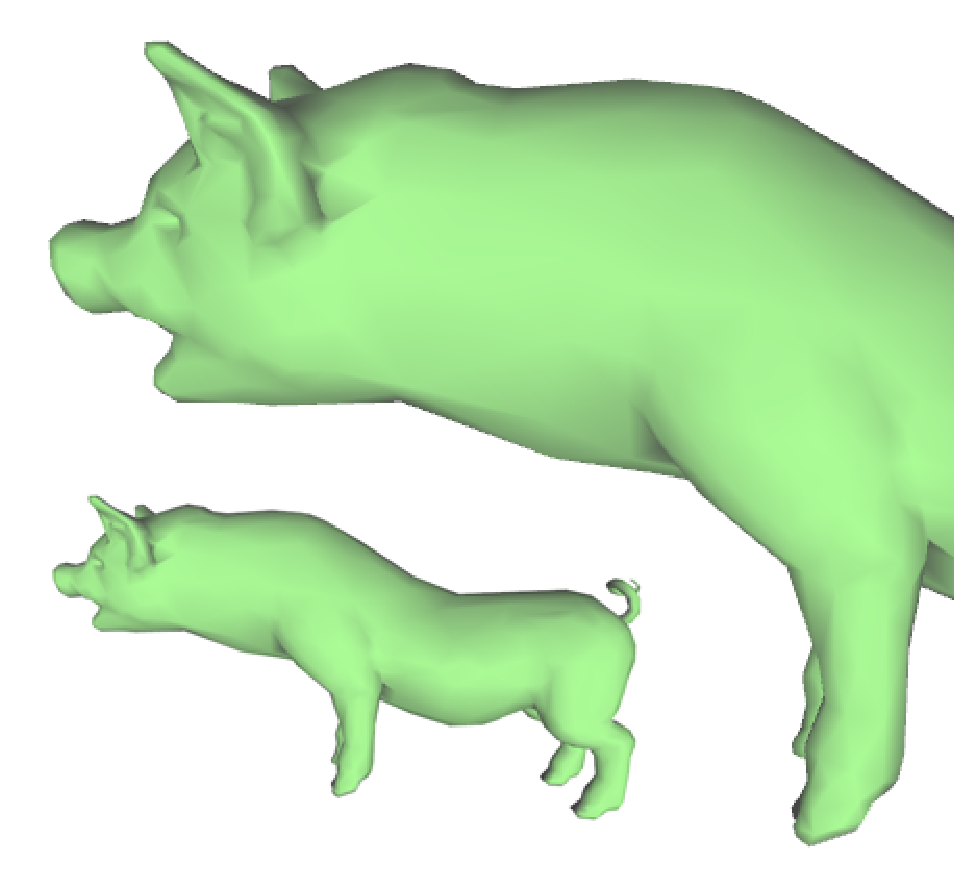
\includegraphics[scale=0.18]{figs/f5.10.PigMat3.eps}
    \end{minipage}}
  \subfigure[]{
    \centering
    \label{fig:deformpig:d}
    \begin{minipage}[b]{0.23\textwidth}
      \centering
      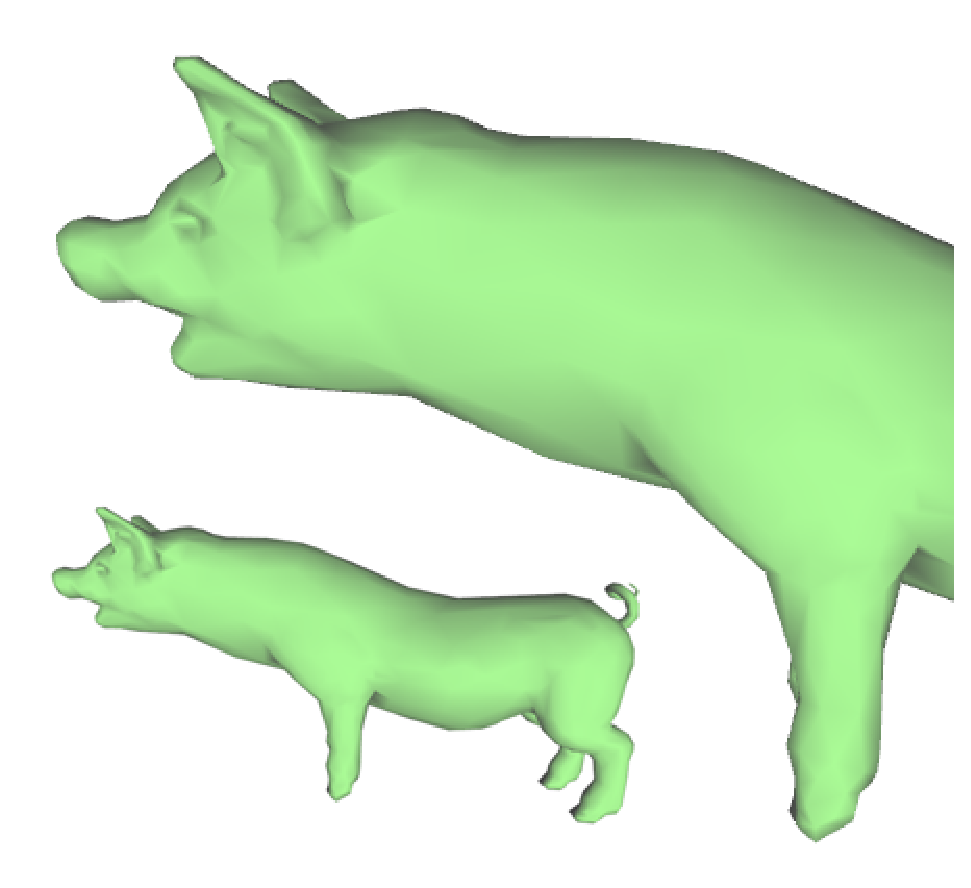
\includegraphics[scale=0.18]{figs/f5.10.PigMat4.eps}
    \end{minipage}}
  \subfigure[]{
    \centering
    \label{fig:deformpig:e}
    \begin{minipage}[b]{0.23\textwidth}
      \centering
      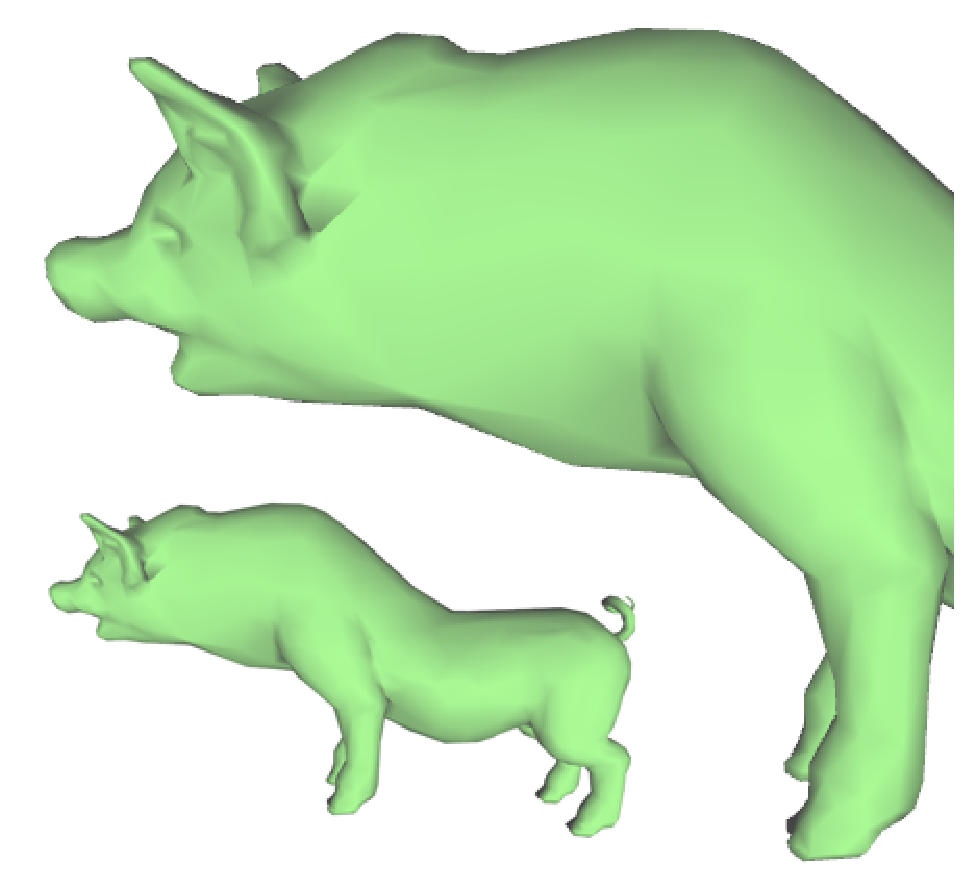
\includegraphics[scale=0.18]{figs/f5.10.PigMat5.eps}
    \end{minipage}}
  \caption{Material-constrained deformation of the \textit{pig} model. (a) The initial model and its specified materials. (b)-(d) Deformation results of uniformly distributed materials with global balance parameter valued 0, 0.5 and 1 respectively. (e) Deformation result with the specified non-uniform materials.}
  \label{fig:deformpig} %% label for entire figure
\end{figure}


It can be summarized that when a globally  consistent deformation is
desired, the global method can be used to produce a well-balanced
result between rigidity and smoothness, subject to the specific
model and user requirement; when the user wants to compute the
deformation of a mesh surface with non-uniformly distributed
materials, then the local method can be used to specify the
stiffness properties of the materials on the local regions and get a
natural and realistic result.


%=================section==================
\section{Results and discussions}
\label{ch5:sec:results}
%==========================================
In our implementation of the proposed  deformation algorithm, the
LAPACK library~\cite{ABBD92} is used to solve the linear equations.
For the operations of the mesh deformation, we adopted a user
interface presented in Chapter~\ref{ch:planeSBIM}, which allows the
user to sketch strokes on the mesh surface and on a reference plane
as the handle curve and its deformed shape (indicated by the blue
and green curves in all the examples) respectively. The ROI is also
specified through sketching. The red dots in the examples indicate
the static vertices.

Figures~\ref{fig:deformbaby}  and~\ref{fig:deformdino} compare the
deformation results of the flexible deformation algorithm performed
directly in the primal domain and via the edge-based graph. In
Figure~\ref{fig:deformbaby} we can see that when $\lambda$ equals 0
or 1, which means a smooth or rigid deformation is requested,
calculations in the primal domain produce poor results: when
$\lambda=0$, the shape of the foot is not well preserved and when
$\lambda=1$, distortions appear around the knee part. However, the
results calculated via the edge-based graph are much better. Similar
observations can be found in Figure~\ref{fig:deformdino}, where the
tail of the dinosaur is lifted and stretched to some extent.

In Figure~\ref{fig:deformbuf}  we stretch the leg of the model and
present different results under various $\lambda$ values. The result
of $\lambda=0$ is quite smooth, but the leg becomes fatter than the
initial one, which means shape preservation is not satisfactory. The
result of $\lambda=1$ preserves the shape well. However, it lacks
some smoothness. The result of $\lambda=0.5$ seems to be the most
natural and realistic one.

Sometimes the most satisfactory  result cannot be easily identified,
such as in the example shown in Figure~\ref{fig:deformJCglb}, in
which we deform the nose of a head model. This is reasonable because
besides the requirement of local feature preservation and global
smoothness, the best deformation also depends on the individual user
preference. From this perspective, all these results are acceptable
and the best is left for the user to choose.

It is also observed that for some  models, the differences between
the deformation results produced through calculating directly in the
primal domain and via the edge-based graph are not quite obvious
when $\lambda=0.5$. This is because the result of $\lambda=0.5$ can
be regarded as a high-level interpolation of those of $\lambda=0$
and $\lambda=1$. Even the results of the pure rigid and smooth
deformations done in the primal domain are far from satisfactory,
interpolation of them may reduce the distortion to some extent.
However, the capability of producing multiple natural and realistic
results under various $\lambda$ values makes the edge-based method
more flexible.

Figures~\ref{fig:deformplane},~\ref{fig:deformJCMat}
and~\ref{fig:deformpig}  show the results of material-constrained
mesh deformation. The deformation results for the same model with
certain uniform materials are also provided for comparisons. In
Figure~\ref{fig:deformplane}, the material at the center part of the
plane is set to be the stiffest and the material in the surrounding
part to be soft. As can be seen, the deformations of these two parts
approximate those of the models with corresponding material
properties. In Figure~\ref{fig:deformJCMat}, we define different
materials on the nose, mouth and face, in order to let the nose
deform rigidly, the face change smoothly, and the mouth change in an
in-between effect. The result looks as if the nose, mouth and face
are transplanted from the models with corresponding uniform
materials. Similar results can be observed on the head, ear and body
of the pig in Figure~\ref{fig:deformpig}, which is an exaggerated
deformation effect often seen in cartoons.

It can be seen that using the  material-constrained deformation
algorithm, we can make the deformation more flexible to produce
different natural and realistic deformation results, which is
usually difficult using previous methods. Comparing with the method
proposed in~\cite{PJS05}, our approach does not require the user to
manually specify the local transformations of the handles and avoids
the translation-insensitivity problem during deformation.

It is worth mentioning that our algorithm  involves a larger linear
system due to the use of the edge-based graph and thus the
computation takes more time. However, in our experiments we found
that the algorithm only needs up to three or four iterations  to
reach convergence, and since only the right hand side of the linear
system needs to be updated at each iteration, the computation is
still  faster than those nonlinear methods.


%=================section==================
%\section{Summary}
%\label{ch5:sec:sum}
%==========================================
%This chapter has proposed to compute mesh deformation through an edge-based graph. The edge-based graph enables a higher sampling rate in shape computation and thus produces better deformation effects especially for coarse mesh models. A mesh deformation model, which combines both the first order and the second order differential quantities, has been proposed. Thus the flexibility of adjusting the deformation results between rigidity and smoothness is obtained. Furthermore, the introduced parameters in the deformation model can be used to control the stiffness property of the surface material. With a simple tool to set the material property, the deformation effects of a mesh with non-uniformly distributed materials can easily be achieved. Experimental results have demonstrated the usefulness of the edge-based graph in mesh deformation and the flexibilities of the proposed deformation algorithm.
